%%%%%%%%%%%%%%%%%%%%%%%%%%%%%%%%%%%%%%%%%%%%%%%%%%%
%
%  New template code for TAMU Theses and Dissertations starting Fall 2016.  
%
%
%  Author: Sean Zachary Roberson
%  Version 3.16.10
%  Last Updated: 9/29/2016
%
%%%%%%%%%%%%%%%%%%%%%%%%%%%%%%%%%%%%%%%%%%%%%%%%%%%

\documentclass[12pt]{report}

%These next lines change the font. Fixes for certain
%fonts will be implemented in a future release.

%Comment this line if you do not wish to use Times
%New Roman. The font used will then be the LaTeX
%default of Computer Modern.
\usepackage{times}
%\usepackage{cmbright}
\usepackage[T1]{fontenc}

%Do not change these settings. The geometry package
%Adjusts the margins to those specified by the Thesis
%Manual. 
\usepackage[letterpaper]{geometry}
\geometry{verbose,tmargin=1.25in,bmargin=1.25in,lmargin=1.4in,rmargin=1.15in}
 \usepackage[doublespacing]{setspace}
 \usepackage{tocloft}
 \usepackage[rm, tiny, center, compact]{titlesec}
 \usepackage{indentfirst}
 \usepackage{etoolbox}

\usepackage{tocvsec2}
 \usepackage[titletoc]{appendix}
 \usepackage{appendix}
 \usepackage{tamuconfig}

\usepackage{rotating}

%These are common AMS packages. Many LaTeX documents
%have these packages declared in their preambles.
\usepackage{amsmath, amsthm}

%This package allows for the use of graphics in the
%document.
\usepackage{graphicx}
\usepackage{subcaption}

%If you have JPEG format images, add .jpg as an
%allowed file extension below. Same for Bitmaps (.bmp).
\DeclareGraphicsExtensions{.png,.jpg,.pdf,.eps}

%It is best practice to keep all your pictures in
%one folder inside the main directory in which your
%TeX file is kept. Here the folder is named "graphic."
%Replace the name here with your folder's name, if needed.
%The period is needed due to relative referencing.
\graphicspath{ {./graphic/} }
\newcommand\figpath{/Users/aperloff/Documents/TAMU-Graduate/Thesis/Text/figures/}

%If needed, this will allow you to add the word "Page"
%to extra pages on your front matter lists.
\usepackage{afterpage}

%This is from the mdwtools package; it fixes some
%footnote commands and allows you to have footnotes in
%tables via the savenotes environment.
\usepackage{footnote}

%This is for sorting tables and displaying their content
\usepackage{datatool}
\usepackage{dataplot}
\usepackage{datapie}
\usepackage{databar}
\usepackage{longtable}
\usepackage{xtab}

\usepackage{cmscommands}

% Added to fix issues with pdf searching in some versions of LaTeX
%\usepackage[T1]{fontenc}\usepackage{lmodern}
%%%%%%%%%%%%%%%%%%%%%%%%%%%%%

% Hyperref setup below.  You should be able to get away with using uncommenting just the first line.
%\usepackage[hidelinks]{hyperref}

% if \usepackage[hidelinks]{hyperref} doesn't work try this.
% \usepackage{hyperref}  % Hidelinks is an option that removes link visiability.  TAMU Thesis Offices prefers to not see the links. But often doesn't work.  
% 
% \hypersetup{
%     colorlinks=true,
%     linkcolor=black,
%     citecolor=black,
%     filecolor=black,
%     urlcolor=black,
% }
%%%%%%%  End of hyperref setup.  One of these two options should work, but my motto with hyperref is when in doubt, comment it out!
%%%%%%%%%  This hopefully fixes the problem with vertical spacing of section headings at the top of the page..  Commented out in 1.0.7
% \preto\section{%
% \ifnum\value{section}>0\addtocontents{toc}{\vskip-6pt}\fi
% }
% \preto\subsection{%
% \ifnum\value{subsection}=0\addtocontents{toc}{\vskip-6pt}\fi
% \ifnum\value{subsection}>0\addtocontents{toc}{\vskip-6pt}\fi
% } 
%%%%%%%%%%%%%%%%%%%%%%%%%%%%%%%%%%%%%%%%%%%%%%%%%%%%%%

\begin{document}

%The title of your document goes here.
%Spacing may need to be adjusted if your title is long
%and pushes the copyright off the page.
\newcommand\hidemath{125 GeV}
\newcommand\hidemathtwo{$H{\rightarrow}WW{\rightarrow}l{\nu}jj$}
\newcommand\hidemaththree{$\sqrt{s}=$\ 8 TeV}
\renewcommand{\tamumanuscripttitle}{Search for a \protect\hidemath\ Standard Model Higgs decaying via \protect\hidemathtwo\ at \protect\hidemaththree}

%Type only Thesis, Dissertation, or Record of Study.
\renewcommand{\tamupapertype}{Dissertation}

%Your full name goes here, as it is in university records. Check your student record on Howdy if there is any mismatch.
\renewcommand{\tamufullname}{Alexx S. Perloff}

%The degree title goes here. See the OGAPS site for more info.
\renewcommand{\tamudegree}{Doctor of Philosophy}
\renewcommand{\tamuchairone}{Ricardo Eusebi}


% Uncomment out the next line if you have co-chairs.  You will also need to edit the titlepage.tex file.
%\newcommand{\tamuchairtwo}{Additional Chair Name}
\renewcommand{\tamumemberone}{Alexei Safonov}
\newcommand{\tamumembertwo}{Bhaskar Dutta}
\newcommand{\tamumemberthree}{Sherry J. Yennello}
\renewcommand{\tamudepthead}{Peter McIntyre}

%Type only May, August, or December.
\renewcommand{\tamugradmonth}{May}
\renewcommand{\tamugradyear}{2017}
%Your department name goes here.
\renewcommand{\tamudepartment}{Physics}


\include{data/titlepage} % This is simply a file that formats and adds your titlepage, please do not edit this unless you have a specific need. .
%!TEX root = ../TAMUTemplate.tex
%%%%%%%%%%%%%%%%%%%%%%%%%%%%%%%%%%%%%%%%%%%%%%%%%%%
%
%  New template code for TAMU Theses and Dissertations starting Fall 2016.  
%
%  Author: Sean Zachary Roberson
%	 Version 3.16.09
%  Last updated 9/12/2016
%
%%%%%%%%%%%%%%%%%%%%%%%%%%%%%%%%%%%%%%%%%%%%%%%%%%%
%%%%%%%%%%%%%%%%%%%%%%%%%%%%%%%%%%%%%%%%%%%%%%%%%%%%%%%%%%%%%%%%%%%%%
%%                           ABSTRACT 
%%%%%%%%%%%%%%%%%%%%%%%%%%%%%%%%%%%%%%%%%%%%%%%%%%%%%%%%%%%%%%%%%%%%%

\chapter*{ABSTRACT}
\addcontentsline{toc}{chapter}{ABSTRACT} % Needs to be set to part, so the TOC doesnt add 'CHAPTER ' prefix in the TOC.

\pagestyle{plain} % No headers, just page numbers
\pagenumbering{roman} % Roman numerals
\setcounter{page}{2}

\indent The Higgs boson discovery was announces on July 4th, 2012. Since then the 125\unit{\GeV} boson has been seen in many decay paths, including $H{\rightarrow}\gamma\gamma$, $H{\rightarrow}ZZ$, $H{\rightarrow}\tau\tau$, and even some $H{\rightarrow}W^{+}W^{-}$ channels.
However, no one has looked for the boson at this mass in the $H{\rightarrow}W^{+}W^{-}{\rightarrow}l{\nu}jj$.
This dissertation presents a search for the 125\unit{\GeV} Higgs in semi-leptonic W decays using both traditional kinetically discriminating variables as well as a matrix element technique.
The data for this analysis was collected in 2012 by the Compact Muon Solenoid (CMS) experiment at the Large Hadron Collider (LHC) and amounts to 19.7\unit{\fbinv} of proton-proton collisions at a center of mass energy of 8\unit{\TeV}.
Although this analysis presents a step forward in complexity, we were still not able to see a significant excess above the standard model background prediction.
However, we were able to set limits on the $\sigma\times{BR}$ for the semi-leptonic W decay of the Higgs boson.
PUT LIMITS HERE.
These represent some of the first such limits recorded.


 

\pagebreak{}


%no bold
%no references or citations
% purpose
% methods
% results
% conclusions

%Contributors and Funding sources required
%dedication and acknowledgments and nomenclature are optional

\include{data/dedication}
%!TEX root = ../TAMUTemplate.tex
%%%%%%%%%%%%%%%%%%%%%%%%%%%%%%%%%%%%%%%%%%%%%%%%%%%
%
%  New template code for TAMU Theses and Dissertations starting Fall 2016.
%
%  Author: Sean Zachary Roberson
%	 Version 3.16.09
%  Last updated 9/12/2016
%
%%%%%%%%%%%%%%%%%%%%%%%%%%%%%%%%%%%%%%%%%%%%%%%%%%%


%%%%%%%%%%%%%%%%%%%%%%%%%%%%%%%%%%%%%%%%%%%%%%%%%%%%%%%%%%%%%%%%%%%%%%
%%                           ACKNOWLEDGMENTS
%%%%%%%%%%%%%%%%%%%%%%%%%%%%%%%%%%%%%%%%%%%%%%%%%%%%%%%%%%%%%%%%%%%%%
\chapter*{ACKNOWLEDGMENTS}
\addcontentsline{toc}{chapter}{ACKNOWLEDGMENTS}  % Needs to be set to part, so the TOC doesnt add 'CHAPTER ' prefix in the TOC.


\indent It's an interesting thing taking stalk of seven years of one's life. To be so grateful to so many people, but be utterly unable to convey the depth of one's gratitude. Nevertheless, that is just how I feel about my time in graduate school.

It has been a true honor to work with my advisor, Professor Ricardo Eusebi. I remember meeting Ricardo at Fermilab when I was an undergraduate summer student, not realizing that this would be a relationship that would enrich my life forever. I have learned an innumerable amount from Ricardo about an ever widening range of topics, from the intricacies of high energy physics, to the navigation of Texas A\&M University regulation, to the benefits of making a solid plan before execution. I am a better student and physicist because of him.

I must also thank the wider TAMU collider physics group for their support and advise. Whether it was a question on physics, career advice, or time on a computing cluster, this group was always there for me. I have spent a significant amount of time at Texas A\&M, so this list is too long to enumerate, but I want each and every one of these people to know that I am forever grateful to them. I am also thankful for our analysis collaborators Professor Chris Neu and Joseph Goodell from the University of Virginia for their invaluable contributions to this analysis. It is a better and more complete analysis because of them. I am also thankful for my fellow physics graduate students. This group of amazing individuals made my time in College Station that much more enjoyable and helped me to grow as a person outside of physics.

Besides my dissertation analysis I have spent many years working for the JetMET/JERC group within CMS. In that time I have worked with countless individuals who should know what a pleasure it was to work alongside them. There are to many names to list here, but there are some which are deserving of explicit recognition: Mikko Voutilainen, Ia Iashvili, Viola Sordini, Hartmut Stadie, Francesco Pandolfi, Salvatore Rappoccio, Philip Harris, Konstantinos Kousouris, and Robert Schoefbeck.

The CMS experiment is a nearly unbelievable undertaking requiring the hard work and dedication of thousands of scientists, engineers, and students. Like everyone else, I owe some portion of my success and results to each and every one of these people. However, I would be remiss if I didn't single out my collaborators and friends from the Fermilab LPC. John Stupak and Ben Kreis, without you I would be a lesser physicist and weaker rock climber than I am today. Kevin Pedro and Lindsay Grey, I can only hope that when I grow up I understand programming languages like you. Nahn Tran, Jim Dolen, and Justin Pilot, thank you for your support on my JEC/JMAR endeavors. Nadja Strobbe, Hansjorge Webber, Scarlet Norber, Joe Prastika, Jamie Antonelli, and Doug Berry, thank you for indulging my never ending and sometimes random questions. I promise they hade a purpose. To everyone else at the LPC, you my everlasting gratitude for your support.

My parents always told me that we collect some relationships from each stage in our lives; that the ones that remain are meant to be. I met Breann Sitarski as undergraduates at UCLA and we remain friends to this day. Each day I am thankful for her friendship and support. And while this may seem like an odd acknowledgment, I know that Breann and I have talked through many analysis challenges and strategies. She is my sounding board.

Finally, I thank my family, whom I love and appreciate more than words can ever describe. My brother Spenser is and always has been my go-to guy. Whether he knows it or not, he is my inspiration and I can only strive to be as engaged and dedicated as he is. My parents Laura and Gregg have supported me throughout this entire graduate process, even when they couldn't understand the title of my dissertation. I am the person I am today...I am here today because of them.

% use A\&M instead of A$\&$M, not use $A\&M$ as well, the last one won't be bold.
%Texas A\&M University


\pagebreak{}
%\include{data/contributors}
%!TEX root = ../TAMUTemplate.tex
%%%%%%%%%%%%%%%%%%%%%%%%%%%%%%%%%%%%%%%%%%%%%%%%%%%
%
%  New template code for TAMU Theses and Dissertations starting Fall 2016.
%
%
%  Author: Sean Zachary Roberson
%	 Version 3.16.09
%  Last updated 9/12/2016
%
%%%%%%%%%%%%%%%%%%%%%%%%%%%%%%%%%%%%%%%%%%%%%%%%%%%

%%%%%%%%%%%%%%%%%%%%%%%%%%%%%%%%%%%%%%%%%%%%%%%%%%%%%%%%%%%%%%%%%%%%%%
%%                           NOMENCLATURE
%%%%%%%%%%%%%%%%%%%%%%%%%%%%%%%%%%%%%%%%%%%%%%%%%%%%%%%%%%%%%%%%%%%%%

\chapter*{NOMENCLATURE}
\addcontentsline{toc}{chapter}{NOMENCLATURE}  % Needs to be set to part, so the TOC doesnt add 'CHAPTER ' prefix in the TOC.

\DTLloaddb{mynomen}{data/nomen.csv}
\dtlsort{abbr=ascending}{mynomen}{\dtlcompare}

\makeatletter
%http://groups.google.com/group/comp.text.tex/msg/7e812e5d6e67fcc5
\def\convertto#1#2{\strip@pt\dimexpr #2*65536/\number\dimexpr 1#1}
\makeatother

%A note about aligning: These entries will align
%themselves according to the ampersand (&).
%No extra spaces are needed, as seen in some of
%the entries below.
\vspace{-0.5in}
	%next two lines remove a problem of adding too much space to the first line
	%\vspace{-\baselineskip}
	\vspace{-\convertto{in}{2ex}in} 
    \begin{longtable}{@{}p{0.33\textwidth} p{0.62\textwidth}@{}}
    \DTLforeach*{mynomen}{}{%
    \\[2ex]\gdef\doamp{\gdef\doamp{&}}%
    \DTLforeachkeyinrow{\thisValue}{\doamp\thisValue}}%
    \end{longtable}%

	%\begin{table}[htbp]
	%    \begin{tabular}{@{}p{0.33\textwidth} p{0.62\textwidth}@{}}
	%	OGAPS	&	Office of Graduate and Professional Studies at Texas A\&M University\\	[2ex]
	%	B/CS		&	Bryan and College Station\\	[2ex] %[2ex] provides double space between each row
	%	TAMU			&	Texas A\&M University\\	[2ex]
	%	AOD     & Analysis Object Data\\ [2ex]
	%	%XXXXXXXX		&	This is an optional page. Random word to test how long the sentence can be? This is just for test purpose. The current setting aims to align left/right margin same as all other pages.\\	[2ex]
	%    \end{tabular}%
	%\end{table}

\pagebreak{}

\include{data/lists}  % This is simply a file that formats and adds your toc, lof, and lot, please do not edit this unless you have a specific need.

%!TEX root = ../TAMUTemplate.tex
%%%%%%%%%%%%%%%%%%%%%%%%%%%%%%%%%%%%%%%%%%%%%%%%%%%
%
%  New template code for TAMU Theses and Dissertations starting Fall 2016.
%
%  Author: Sean Zachary Roberson 
%	 Version 3.08.16
%  Last updated 8/19/2016
%
%%%%%%%%%%%%%%%%%%%%%%%%%%%%%%%%%%%%%%%%%%%%%%%%%%%

%%%%%%%%%%%%%%%%%%%%%%%%%%%%%%%%%%%%%%%%%%%%%%%%%%%%%%%%%%%%%%%%%%%%%%
%%                           SECTION I
%%%%%%%%%%%%%%%%%%%%%%%%%%%%%%%%%%%%%%%%%%%%%%%%%%%%%%%%%%%%%%%%%%%%%


\pagestyle{plain} % No headers, just page numbers
\pagenumbering{arabic} % Arabic numerals
\setcounter{page}{1}


\chapter{\texorpdfstring{\uppercase {Introduction}}{Introduction}}
\begin{comment}
1) Physics/colliders
2) Standard model
3) Higgs
4) This dissertation toppic
5) Organization
\end{comment}

Particle physicists seek to understand the building blocks of the universe and how they interact.
An understated search to characterize the fundamental constituents of nature which can be built up into the world we see.
In this quest there has been no better tool than the synchrotron, a circular accelerator which collides particles at speeds approaching that of light.
As the accelerators reach higher and higher energies, physicists are able to probe smaller distance scales and even create heavy, short lived particles which are otherwise inaccessible.
The standard model (SM) of particle physics is the codification of over a century of study.
It describes all of the observed elementary particles, their properties, and the electromagnetic, weak, and strong forces through which they interact.
The standard model, a specific framework born out of quantum field theory (QFT), has predicted quantities and been proven accurate time and time again.
Yet until recently it remained an incomplete model, at least experimentally.

One of the primary missions of the Large Hadron Collider (LHC), the worlds highest energy particle accelerator located at the European Organization for Nuclear Research (CERN), was to search for the last remaining particle in the SM.
On July 4th, 2012 the ATLAS (A Toroidal LHC Apparatus) and CMS (Compact Muon Solenoid) collaborations at the LHC simultaneously confirmed the discovery of a new boson~\cite{20121,201230}.
Since its discovery, the particle has been shown to be consistent with the long proposed the Higgs boson, said to give mass to itself and all of the other massive particles through the process of electroweak symmetry breaking.
It took almost 50 years for experimentalists to confirm the existence of the boson first proposed in 1964 as the spin zero mediator to the standard models only scalar field.

Using 19.7\fbinv of 8\tev data from the CMS experiment at CERN, the Higgs boson mass was measured to be \longmass{125.7}{0.3}{0.3}{\gev}\footnote{Unless otherwise indicated this document will use natural units, where $c=\hbar=1$.}\footnote{This measurement has subsequently been improved by combining the ATLAS and CMS measurements. The measured Higgs mass as of 2015 was \longmass{125.09}{0.21}{0.11}{\gev}~\cite{Aad:2015zhl}.} by five major decay modes: $H\rightarrow\gamma\gamma$, $H\rightarrow\tau\tau$, $H\rightarrow{bb}$, $H\rightarrow{ZZ}$, and $H\rightarrow{WW}$~\cite{CMS-PAS-HIG-13-005}.
Since then, the experiment has entered a phase of intense study of the new particle.
Every property of the new boson and all of its decay channels must be studies in great detail to confirm that it is indeed the SM Higgs boson and not a very similar particle.
Currently the properties of the new boson are consistent with those predicted by the SM, but any deviation from the SM predictions could point to some new, as yet unexplored physics.

This dissertation will present a search for the 125\gev Higgs boson in the the\newline\HWWlnujj decay channel using 8\tev proton-proton data collected by the CMS detector.
Although the \HWWlnujj channel was used in the original combined limit, the previous search was not sensitive to the ``low mass'' Higgs, but only to 
$\MH>2\MW$~\cite{CMS-PAS-HIG-13-027}.\footnote{The lowest search mass was $\MH=170\gev$.}
Because the Higgs mass is less than two times the mass of the W boson, at least one of the W bosons must be created ``off-shell'', meaning that its measured mass is not $\sim80\gev$.
On top of that, the presence of a neutrino makes it a challenge to fully reconstruct the initiating particle.
For these reasons the $WW\rightarrow{l\nu}{l\nu}$ decay channel was the most sensitive of the $WW$ channels during the 2012 combination.
Nevertheless this analysis will search for the low mass Higgs boson in the semi-leptonic channel using a matrix element (ME) technique to boost the signal extraction sensitivity.

This dissertation will be organized in the following way.
Chapter~\ref{ch:theoretical_framework} will present an overview of the standard model, the Higgs mechanism, and a brief introduction to how the Higgs can point to physics beyond the standard model (BSM).
The LHC and CMS will be described in chapter~\ref{ch:LHC_CMS}.
Chapter~\ref{ch:event_reconstruction} describes the reconstruction of an event at CMS and all of the final physics objects.
Chapter~\ref{ch:analysis} discusses the analysis work-flow from data samples used to signal extraction techniques while the results are presented in chapter~\ref{ch:results}.
Chapter~\ref{ch:conclusion} gives some concluding remarks.


%!TEX root = ../TAMUTemplate.tex
%%%%%%%%%%%%%%%%%%%%%%%%%%%%%%%%%%%%%%%%%%%%%%%%%%%
%
%  New template code for TAMU Theses and Dissertations starting Fall 2016.
%
%  Author: Sean Zachary Roberson
%	 Version 3.16.09
%  Last updated 9/12/2016
%
%%%%%%%%%%%%%%%%%%%%%%%%%%%%%%%%%%%%%%%%%%%%%%%%%%%

%%%%%%%%%%%%%%%%%%%%%%%%%%%%%%%%%%%%%%%%%%%%%%%%%%%%%%%%%%%%%%%%%%%%%%%
%%%                           SECTION II
%%%%%%%%%%%%%%%%%%%%%%%%%%%%%%%%%%%%%%%%%%%%%%%%%%%%%%%%%%%%%%%%%%%%%%


\chapter{\uppercase {The LHC and CMS Detector}}
\label{ch:LHC_CMS}

\section{The Large Hadron Collider}
\label{sec:LHC}

The Large Hadron Collider (LHC) \cite{Breskin:1244506} is, in many people's estimation, the largest and most complex machine ever built by humanity.
The main accelerator at the European Organization for Nuclear Research (CERN), the LHC is located both in France and Switzerland due to its enormous size (Fig.~\ref{fig:LHC_schematic}).
It was built between 1998 and 2008 and installed in the 26.7\unit{km} tunnel dug for its predecessor, the Large Electron-Positron Collider (LEP), which is located between 50\unit{m} and 170\unit{m} underground.
It is the highest energy collider in the world, eclipsing the previous record holder, the Tevatron at Fermilab in Batavia, IL.
The following section is a description of the LHC and CERN accelerator complex based on \cite{LHCmachine} and \cite{Breskin:1244506}.

\begin{figure}[!hbt]
	\vspace*{-0.5cm}
	\centering
	\includegraphics[width=0.95\textwidth]{\figpath/Chapter2/LHC_schematic.jpg}
	\caption{Overhead view of CERN and its main experiments, CMS; ATLAS; LHCb; and ALICE, as well as two of the larger accelerators, the LHC and SPS. The schematic is overlaid on a map of Switzerland and France~\cite{LHC-schematic}.}
	\label{fig:LHC_schematic}
\end{figure}

The LHC provides beams for four main experiments located along its beam line (Fig.~\ref{fig:LHC_schematic}):
\begin{itemize}
	\item The CMS (Compact Muon Solenoid)~\cite{Chatrchyan:2008aa} and ATLAS (A Toroidal LHC ApparatuS)~\cite{1748-0221-3-08-S08003} experiments are both general purpose detectors. Their goals include precision measurements to test the Standard Model and searches for new physics, including the Higgs boson.
	\item LHCb (Large Hadron Collider beauty)~\cite{Alves:2008zz} was designed to do precision measurements of CP-violation and the physics of B-mesons.
	\item ALICE (A Large Ion Collider Experiment)~\cite{Aamodt:2008zz} studies heavy ion collisions.
\end{itemize}

The LHC was designed to collide two beams of protons (pp), heavy ions (PbPb), or a combination of the two (pPb) at specific interaction points around the beam line.
For the purposes of this thesis we will only cover proton-proton collisions from this point forward.
The protons come from a single bottle of hydrogen gas, which is then disassociated and stripped of electrons to form a proton beam.
Interestingly, only 1\unit{ng} of hydrogen is required per day in order to form the LHC beams.
The protons next travel through the Linac2 machine where they form bunched by radio frequency (RF) electromagnetic fields and are accelerated to 50\MeV.
This chain continues through the Proton Synchroton Booster (PSB), the Proton Synchrotron (PS), and the Super Proton Synchrotron (SPS) where the protons are accelerated to 1.4\GeV, 26\GeV, and 450\GeV respectively (Fig.~\ref{fig:CERN_accelerators}).

\begin{sidewaysfigure}[!hbt]
	\centering
	\begin{subfigure}[t]{0.4655\textwidth}
		\includegraphics[width=\textwidth]{\figpath/Chapter2/CERN's-accelerator-complex2013.jpg}
		\label{fig:CERN_accelerator_complex}
	\end{subfigure}
	\begin{subfigure}[t]{0.4655\textwidth}
		\includegraphics[width=\textwidth]{\figpath/Chapter2/lhc-pho-1993-008.png}
		\label{fig:LHC_LEP_injection_complex}
	\end{subfigure}
	\caption{Left: A schematic of the CERN accelerator complex~\cite{Marcastel:1621583}. Right: A diagram of the LHC injection chain. Also included is a diagram of the heavy ion and LEP injection chains~\cite{Jean-Luc:841568}.}
	\label{fig:CERN_accelerators}
\end{sidewaysfigure}

\clearpage

After being accelerated in the SPS, the proton bunches are injected into the two LHC beam pipes, which were designed to accelerate the two proton beams to 7\TeV (Fig~\ref{fig:LHC_beams}).
Size limitations in the tunnel dictated that the the beam lines be formed by twin bore magnets.
Each magnet is formed by a single mechanical structure and cryostat while containing two coils and two beam channels.
The coils are made out of superconducting NbTi Rutherford cables cooled to 1.9\unit{K} by 120\unit{t} of superfluid helium.
This forms the 8.33\unit{T} magnets necessary for bending the 7\TeV protons (Fig.~\ref{fig:LHC_magnet}).
The LHC contains 1232 superconducting dipole magnets for bending the protons and 392 superconducting quadrupole magnets for focusing the beams.
The beam line also contains sextapole, octopole, and decapole magnets, which are also used to correct and focus beams.
The original LHC design calls for a bunch spacing of 25\unit{ns}, $10^{11}$ protons per bunch, and 2808 bunches per beam.
%The acceleration is accomplished by 16 RF cavities operating at 400MHz.

\begin{figure}[!hbt]
	\centering
	\includegraphics[width=0.95\textwidth]{\figpath/Chapter2/lhc-pho-1997-060.png}
	\caption{A diagram of the LHC beams along with the four major experiments~\cite{Jean-Luc:841573}.}
	\label{fig:LHC_beams}
\end{figure}

\begin{figure}[!hbt]
	\centering
	\includegraphics[width=0.95\textwidth]{\figpath/Chapter2/lhc-pho-1998-299.jpg}
	\caption{A diagram of an LHC dipole magnet and cryostat~\cite{Dailler:842253}.}
	\label{fig:LHC_magnet}
\end{figure}

The original plan was to start the LHC accelerator complex in September 2008.
However, due to a catastrophic incident damaging the machine, the startup was delayed until November 23, 2009; even then colliding beams only had a center-of-mass energy of 900\GeV.
From March 30, 2010 through the end of 2011 the LHC operated with a center-of-mass energy of 7\TeV.
Then in 2012 the energy was again increased to 8\TeV (4\TeV per beam), which is the energy of the beams during the data-taking period focused on by this thesis.
It is important to note, though, that the machine has continued to operate after the 2012 data taking period and increased the center-of-mass energy to 13\TeV starting in 2015 (there was a planned shutdown from 2013 through early 2015).

In addition to the center-of-mass energy, collider physicists are interested in the rate at which a specific physics process occurs.
This in turn is related to the cross sections, the probability that two particles will collide and react a certain way, and the luminosity.
The rate of events is given by equation~\ref{eq:dn/dt}, where $\mathcal{L}$ is the collision luminosity and $\sigma$ is the cross section for a given physical process.

\begin{equation}
dN/dt=\mathcal{L}{\cdot}\sigma
\label{eq:dn/dt}
\end{equation}

The luminosity as it is described here is often called the ``instantaneous luminosity'' as this value can change from moment to moment.
The ``integrated luminosity'' is then a measure of the total amount of data collected.
The instantaneous luminosity itself depends upon the parameters of the LHC beams and the optical properties of the focusing system at the interaction point.
This information is summed up in equation~\ref{eq:luminosity}~\cite{1742-6596-455-1-012001}:

\begin{equation}
\mathcal{L}=\frac{N^{2}n_{b}f\gamma}{4\pi\epsilon_{n}\beta^{*}}F
\label{eq:luminosity}
\end{equation}

where:

\begin{itemize}
	\item $N$: protons per bunch
	\item $n_{b}$: bunches in the LHC ring
	\item $f$: frequency of bunch revolutions around the ring 
	\item $\gamma$: relativistic factor for the protons
	\item $\epsilon_{n}$: normalized emittance of the proton beams
	\item $\beta^{*}$: beta function at the interaction point
	\item $F$: geometrical reduction factor due to the crossing angle of the beams
\end{itemize}

The maximum design luminosity of the LHC is $1\times10^{34}\percms$.
During the 2010 and 2011 run periods (7\TeV center-of-mass energy) the instantaneous luminosity increased from $1\times10^{32}\percms$ to $5\times10^{33}\percms$.
During the 2012 data-taking period, the peak instantaneous luminosity was $7.67\times10^{33}\percms$ with a bunch spacing of 50\unit{ns}, a maximum number of bunches of 1380, and $\sim2.2\times10^{14}$ protons per beam ($\sim1.6\times10^{11}$ protons per bunch).
The LHC delivered 23.30\fbinv of integrated luminosity to the CMS detector of which 21.79\fbinv was recorded.
As of the end of 2016, the LHC is still running at 13\TeV (6.5\TeV per beam) with a peak luminosity of $1.53\times10^{34}\percms$, 2208 bunches, and $1\times10^{11}$ protons per bunch~\cite{CMSWebBasedMonitoring,LumiPublic}.
Figures~\ref{fig:LHC_int_lumi_pp} and~\ref{fig:LHC_lumi_per_day_pp} show the total integrated luminosity delivered by the LHC and recorded by the CMS experiment for the various data-taking periods~\cite{LumiPublic}.

\begin{figure}[!hbt]
	\centering
	\includegraphics[width=0.95\textwidth]{\figpath/Chapter2/int_lumi_cumulative_pp_2.pdf}
	\caption{Total integrated luminosity versus time delivered to the CMS experiment for the 2010, 2011, 2012, 2015, and 2016 p-p data-taking periods~\cite{LumiPublic}.}
	\label{fig:LHC_int_lumi_pp}
\end{figure}

\begin{figure}[!hbt]
	\centering
	\includegraphics[width=0.95\textwidth]{\figpath/Chapter2/int_lumi_per_day_cumulative_pp_2012.pdf}
	\caption{Total integrated, offline luminosity versus day in 2012. The blue graph shows the delivered luminosity while the orange graph shows the luminosity recorded by the CMS experiment. This graph shows only the luminosity collected for p-p collisions during stable beams~\cite{LumiPublic}.}
	\label{fig:LHC_lumi_per_day_pp}
\end{figure}


\section{The CMS Detector}

TALK ABOUT THE PHYSICS GOALS?
%"The physics program of the experiment covers a wide range of goals: precision study of Standard Model processes, study of properties of the recently discovered Higgs boson, searches for physics beyond the Standard Model, and study of quark-gluon plasma." - Aysen Tatarinov

The CMS experiment is one of two general purpose detectors at the LHC; ATLAS being the other one.
The detector is located 100\unit{m} underground near Cessy, France on the opposite side of the LHC from the main CERN site in Meyrin (see figure~\ref{fig:LHC_schematic}).
It was largely built on the surface and then lowered into the collision cavern in 15 pieces, which then had to be painstakingly assembled.
The detector has a cylindrical design which is 22\unit{m} in length, 15\unit{m} in diameter, and weights 14000 tonnes.
The shape and positioning of the detector around the interaction point (IP) gives the experiment nearly $4\pi$ coverage of the proton collisions.
The layout of the detector can be seen in fig.~\ref{fig:CMS_schematic}.

\begin{figure}[!hbt]
	\centering
	\includegraphics[width=0.95\textwidth]{\figpath/Chapter2/cms_160312_02.png}
	\caption{Schematic of the CMS detector with labels and notable figures~\cite{SketchUpCMS}.}
	\label{fig:CMS_schematic}
\end{figure}

Fig.~\ref{fig:CMS_transverse} shows how various types of particles interact within the CMS sub-detectors.
In total, there are ${\sim}10^8$ data channels checked in each bunch crossing owing to the high granularity of the CMS sub-detectors.
The following sections will describe each of the sub-detectors and its properties and is based largely on Ref.~\cite{Chatrchyan:2008aa}.

\begin{figure}[!hbt]
	\centering
	\includegraphics[width=0.95\textwidth]{\figpath/Chapter2/CMS_slice.png}
	\caption{Transverse slice of the CMS experiment with the major sub-detectors and components represented. The different colored lines represent how various types of particles interact with the sub-detectors~\cite{CMSSlice}.}
	\label{fig:CMS_transverse}
\end{figure}

\subsection{Coordinate System}

The IP is at the center of the detector and is the origin of the right-handed coordinate system used to describe the detector and the physics being measured (location and direction).
The $z$-axis is defined along the LHC beam line.
Instead of using the polar angle, $\theta$, which would go from $0^{\degree}$ along the positive $z$-axis to $90^{\degree}$ pointing straight up from the interaction point, collider physicists use the quantity pseudorapidity defined as $\eta=-ln\left[\tan\left(\theta/2\right)\right]$.
The benefits of using the pseudorapidity are that differences in this coordinate, $\Delta\eta$, are invariant under boosts in the $z$-direction and particle production is roughly uniform in $\eta$.
The $x$- and $y$-axes form the plane perpendicular to the $z$-axis, where positive $x$ points to the center of the LHC ring and positive $y$ points upward.
The azimuthal angle, $\varphi$, and radial coordinate, $r$, are also defined in this same plane.
It is sometimes more useful to use $\varphi$ and $r$ due to the bending of the particles in the magnetic field.
Lastly, this paper will often refer to the quantity \pt, which is the magnitude of the component of the momentum vector in the transverse plane.
A schematic of the coordinate system described above is shown in fig.~\ref{fig:CMS_coordinate_system}.

\begin{figure}[!hbt]
	\centering
	\includegraphics[width=0.95\textwidth]{\figpath/Chapter2/Figures_T_Coordinate.png}
	\caption{Schematic of the CMS coordinate system~\cite{Schott:2014sea}.}
	\label{fig:CMS_coordinate_system}
\end{figure}

\subsection{Tracker and Pixel Detector}
\label{sec:tracker_and_pixel}

The CMS all-silicon tracker is the closest sub-detector to the LHC beam pipe.
Its purpose is twofold; to determine the charged-particle direction at its production vertex and to measure the momentum of charged particles.
In the later case, the tracker is far superior to the calorimeter systems for \pt up to several hundred \gev.
The sub-detector is 5.8\unit{m} long and 2.5\unit{m} in diameter, covering a pseudorapidity range of $\abs{\eta}<2.5$.
It is, by necessity, highly granular, to keep the occupancy low, and relatively radiation hard.
The tracker is exposed to extreme doses of radiation ranging from 0.18 to 84\unit{Mrad} after 500\fbinv of data.
The radiation tolerance was a key factor in determining the materials and design of the sensors and on-board electronics of the tracker.
To keep the radiation damage as low as possible, among other benefits, the tracker is kept at $-10\degC$.
For non-isolated particles of $1<\pt<10\GeV$ and $\abs{\eta}<1.4$, the track resolutions are typically 1.5\% in \pt and 25--90 (45--150)\mum in the transverse (longitudinal) impact parameter.
On the other hand, isolated particles of $\pt=100\GeV$ emitted at $\abs{\eta}<1.4$ have track resolutions of 2.8\% in \pt and 10 (30)\mum in the transverse (longitudinal) impact parameter~\cite{TRK-11-001}.
At higher $\eta$ the reduced transverse depth of the tracker degrades the resolution (particles traverse fewer layers).
Fig.~\ref{fig:CMS_tracker} shows the layout of the tracker and its subsystems. The tracker is formed by two major subsystems, the pixel detector and the silicon strip tracker.


\begin{figure}[!hbt]
	\centering
	\includegraphics[width=0.95\textwidth]{\figpath/Chapter2/CMS_tracker.pdf}
	\caption{Layout of the CMS tracker with subsystems labeled.}
	\label{fig:CMS_tracker}
\end{figure}

The pixel detector is made up of three barrel layers, called the BPIX, and two endcap layers called the FPIX.
The BPIX contains 48 million pixels and the FPIX contains another 18 million pixels.
In total it consists of 1440 hybrid silicon detector modules, each with a dimension of $100\times150\mum^{2}$.
The small pixel size enables track resolutions of 10\mum in the transverse plane and 20\mum in the $z$-direction.
The pixel detector is what gives CMS its excellent secondary vertex tagging ability in addition to producing seed tracks for the strip tracker and the high level trigger.
NOT SURE I LIKE THIS LAST SENTENCE

Just as the pixel detector was made up of the BPIX and FPIX subsystems, the silicon strip detector is made up of four subsystems.
The Tracker Inner Barrel
(TIB) has four layers of 320\mum strips.
At each end of the TIB is a three-layer Tracker Inner Disks (TID), which contains strips of the same thickness.
The Tracker Outer Barrel (TOB) is the six layer system which surrounds the TIB/TID.
The first four layers of the TOB use 500\mum thick strips, and the last two layers use 122\mum thick strips.
The Tracker EndCaps (TEC) are on either side of the previous setup and contains nine disks with up to seven layers of strips.
These strips are 320\mum thick in the inner four rings and 500\mum thick in the outer three rings.
In total, the strip detector contains 9.3 million silicon strips (15\,148 modules).

The 2012 LHC run was an excellent year for the tracker.
The BPIX maintained 97.7\% of its channels operational while the FPIX had 92.8\% of its channels operational.
The reconstruction efficiencies were also quite high, 99.5\%, for each later of the pixel detector ($>$99.2\% for the first layer).
The strip detector maintained 97.5\% of its channels active and had a reconstruction efficiency greater than 99\% for each layer\cite{Veszpremi:2014hpa}. 

\subsection{Electromagnetic Calorimeter}

The electromagnetic calorimeter (ECAL) is a homogeneous detector consisting entirely of 75\,848 lead tungstate crystals (\PbWO).
The detector is divided up into two sections which provide coverage in pseudorapidity \absetalt{1.479} in a barrel region (EB) and \abseta{1.479}{3.0} in two endcap regions (EE).
There are also preshower detectors (PS) in each of the endcaps, in front of the EE, which cover a pseudorapidity range of \abseta{1.653}{2.6}.
Fig.~\ref{fig:CMS_ECAL} shows the structure of the detector with the key $\eta$ values labeled.

\begin{figure}[!hbt]
	\centering
	\includegraphics[width=0.95\textwidth]{\figpath/Chapter2/ECAL_transverse_section.pdf}
	\caption{A schematic of the CMS ECAL detect with labeled subsystems and key $\eta$ ranges marked.}
	\label{fig:CMS_ECAL}
\end{figure}

The barrel region of the ECAL consists of 61\,200 crystals with a tapered shape arranged in a projective geometry. Each crystal is about \mytimes{0.0174}{0.0174} in $\eta-\varphi$, which corresponds to \mytimes{22}{22}\unit{mm$^{\text{2}}$} at the front face and \mytimes{26}{26}\unit{mm$^{\text{2}}$} at the back face. Each crystal has a depth of 230\mm, which for \PbWO corresponds to 25.8 radiation lengths ($X_{0}$). The scintillation light produced in the crystals is read out by avalanche photodiodes (APDs), which produce approximately 4.5 photoelectrons per \MeVns at 18\degC. The dark current of the APDs is sensitive to radiation exposure. During the 2012 run, the dark current ranged from 0.13 to 1.3\muA on average, which corresponds to an average noise of 47 to 57\mev~\cite{CMS:2013ecal}.

The EE contains 14\,648 \PbWO crystals arranged in a non-projective $x-y$ geometry (see fig.~\ref{fig:CMS_ECAL}). The crystal dimensions are \mytimes{28.62}{28.62}\unit{mm$^{\text{2}}$} at the front face and \mytimes{30}{30}\unit{mm$^{\text{2}}$} at the back face with a depth of 220\mm or 24.7 $X_{0}$. Instead of using APDs link in the EB, the EE uses vacuum phototriodes (VPTs) to read out the scintillation light. Again holding the photodetectors at 18\degC, the phototriodes produce 4.5 photoelectrons per \MeVns. The average noise in the VPTs for 2012 was 180--200\mev, but it could reach 600\mev at high $\eta$ due to the higher radiation doses in the more forward regions~\cite{CMS:2013ecal}.

The ES is located in front of each of the EE detectors. It consists of two planes of silicon strip sensors interleaved with a total of $3 X_0$ of lead absorber (2 $X_{0}$ for the first layer and 1 $X_{0}$ for the second layer). The silicon strips are 320\mum thick and can collect 3.6\unit{fC} of charge from a minimum ionizing particle (MIP).

One of the main goals of the CMS experiment was to discover the Higgs boson.
Because of its low irreducible standard model background, the $H\rightarrow\gamma\gamma$ channel was considered the ``golden channel''.
Due to this, a significant amount of money and time was spent on the design and the materials for the ECAL.
\PbWO is a great choice for an ECAL because its properties, listed in table~\ref{tab:PbWO4Properties}, lead to a precision energy measurement for EM objects (by this I mean a fine small resolution). 

\DTLnewdb{PbWO4Data}
\DTLnewrow{PbWO4Data}%
\DTLnewdbentry{PbWO4Data}{Property}{Peak emission wavelength}%
\DTLnewdbentry{PbWO4Data}{Value}{425\unit{nm}}%
\DTLnewrow{PbWO4Data}%
\DTLnewdbentry{PbWO4Data}{Property}{High density}%
\DTLnewdbentry{PbWO4Data}{Value}{8.28\unit{g/cm$^{\text{3}}$}}%
\DTLnewrow{PbWO4Data}%
\DTLnewdbentry{PbWO4Data}{Property}{Short radiation length}%
\DTLnewdbentry{PbWO4Data}{Value}{0.89\unit{cm}}%
\DTLnewrow{PbWO4Data}%
\DTLnewdbentry{PbWO4Data}{Property}{Short Moli\`{e}re radius}%
\DTLnewdbentry{PbWO4Data}{Value}{2.2\unit{cm}}%
\DTLnewrow{PbWO4Data}%
\DTLnewdbentry{PbWO4Data}{Property}{Fast decay time}%
\DTLnewdbentry{PbWO4Data}{Value}{6\unit{ns}}%
%\dtlsort{Property}{PbWO4Data}{\dtlcompare}

\begin{table}[htbp]
\caption{\PbWO properties and their measured values}
\centering
\begin{tabular}{|l|c|}%
\dtldisplaystarttab
Property & Value %
\DTLforeach
*
{PbWO4Data}{}{%
\gdef\doamp{\gdef\doamp{&}}%
\DTLiffirstrow{\\\hline}{\\}%
\DTLforeachkeyinrow{\thisValue}{\doamp\thisValue}}%
\dtldisplayendtab
\end{tabular}
\label{tab:PbWO4Properties}
\end{table}

The energy resolution, $\sigma$, of deposits in the ECAL vary as a function of energy ($E$) (in units of \unit{\gev}).
This is typically modeled using an NSC function as in equation~\ref{eq:ECAL_NSC}:

\begin{equation}
\label{eq:ECAL_NSC}
\left(\frac{\sigma}{E}\right)^{2}=\left(\frac{N}{E}\right)^{2}+\left(\frac{S}{\sqrt{E}}\right)^{2}+C^{2}
\end{equation}

\noindent where $N$ is the noise term, $S$ is the stochastic term, and $C$ is the constant term.
Typical values for these terms come from test beam studies and are listed in table~\ref{tab:ECAL_NSC}~\cite{CMS:2013ecal}.
In the barrel section of the ECAL, an energy resolution of about 1\% is achieved for unconverted or late-converting photons in the tens of GeV energy range.
The remaining barrel photons have a resolution of about 1.3\% up to a pseudorapidity of \absetaeq{1}, rising to about 2.5\% at \absetaeq{1.4}.
In the endcaps, the resolution of unconverted or late-converting photons is about 2.5\%, while the remaining endcap photons have a resolution between 3\% and 4\%~\cite{CMS:EGM-14-001}.

\begin{table}[htbp]
\caption{Typical values for the noise, stochastic, and constant terms of the ECAL energy resolution function. These values are obtained from test beam studies.}
\centering
\begin{tabular}{|l|c|}%
\hline %
Term & Typical Value \\%
\hline
N & 12\% \\%
S & 2.8\% \\%
C & 0.30\% \\%
\hline
\end{tabular}
\label{tab:ECAL_NSC}
\end{table}

\subsection{Hadron Calorimeter}
\label{sec:hadron_calorimeter}

The CMS hadron calorimeter (HCAL) is, as its name suggests, designed to measure the energy of hadrons.
This is especially important for neutral hadrons which leave no tracks and, to a large extent, do not register in the ECAL.
The HCAL is a sampling calorimeter, meaning that is contains both an active, energy measurement material as well as a material which induces the hadrons to shower.
The HCAL is made up of four subsystem: HCAL barrel (HB), HCAL endcap (HE), HCAL outer (HO), and HCAL forward (HF).
The HB, HE, and HO subsystems all use the same technology, while the HF uses a different technology.
Fig.~\ref{fig:CMS_HCAL} shows the structure and position of the HCAL subsystems.
When both the ECAL and HCAL work together, the CMS calorimeters can measure a charged pion with a resolution of $\sigma/E\approx100\%/\sqrt{E[GeV]}\oplus5\%$, where $E$ is the jet energy.

\begin{figure}[!hbt]
	\centering
	\includegraphics[width=0.95\textwidth]{\figpath/Chapter2/HCAL_subdet.pdf}
	\caption{A schematic of the CMS HCAL detector with its major subsystems labeled: HB, HE, HO, and HF.}
	\label{fig:CMS_HCAL}
\end{figure}

The HB occupies the region \absetalt{1.3} and contains alternating layers of brass and scintillator.
The number of nuclear interaction lengths ($\lambda_{0}$) ranges from 5.82 at $\eta=0$ to 10.6 at $\eta=1.3$.
Additionally the EB, which is directly in front of the HB, has 1.1$\lambda_{0}$ and can measure a portion of early developing hadronic showers, though not as accurately.
The properties of the brass used can be found in table~\ref{tab:HCAL_brass_properties} while the layer thicknesses and materials can be found in table~\ref{tab:HCAL_brass_thickness}.
Most of the plastic scintillating layers are 3.7\unit{mm} thick, but layer 16 is 9\unit{mm} thick so that is can sample more from late developing showers.
There is also an additional 9\unit{mm} thick layer 0 before the first absorbing layer so catch the showers which are initiated in the dead material between the EB and HB.
The scintillating tiles are arranged in a projective geometry (pointing close to the nominal interaction point) with the tiles occupying \mytimes{0.087}{0.087} in $\eta-\varphi$.
For \absetalt{1.479}, the HCAL cells map on to $5\times5$ arrays of ECAL crystals to form calorimeter towers.
Within each tower, the energy deposits in ECAL and HCAL cells are summed to define the calorimeter tower energies, subsequently used to provide the energies and directions of hadronic jets.
The scintillator is separated into 16 $\eta$ section and 36 $\varphi$ sections with almost 70000 tiles used.
The light is collected by wavelength shifting (WLS) fibers that encircle the tiles.
Fibers from several layers are read out by one hybrid photodiode (HPD), which are used for their large dynamic range and low sensitivity to magnetic fields.

\begin{table}[htbp]
\caption{Properties of the brass absorber used for the CMS HB.}
\centering
\begin{tabular}{|l|c|}%
\hline %
Property & Value \\%
\hline
Materials & Brass (70\% Copper and 30\% Zinc) or Steel \\%
Density & 8.53\unit{g/cm$^{\text{3}}$}\% \\%
Radiation Length & 1.49\unit{cm} \\%
Nuclear Interaction Length & 16.42\unit{cm}\\
\hline
\end{tabular}
\label{tab:HCAL_brass_properties}
\end{table}

\begin{table}[htbp]
\caption{Absorbing layer thicknesses and materials for the CMS HB}
\centering
\begin{tabular}{|l|c|c|}%
\hline %
Layer number(s) & Material & Thickness (\unit{mm}) \\%
\hline
1 & Steel & 40 \\%
2-9 & Brass & 50.5 \\%
10-15 & Brass & 56.5 \\%
16 & Steel & 75 \\%
\hline
\end{tabular}
\label{tab:HCAL_brass_thickness}
\end{table}

In the central region of the detector there are too few $\lambda_{0}$ to fully contain a hadronic shower.
For this reason the HO system was added as a scintillating tile extension to the HB.
The HO consists of five rings, each with a width of 2.536\unit{m} in the $z$-direction.
The most central ring, Ring 0, has two scintillating layers, one inside the solenoid and one outside the solenoid.
The other rings have only one layer outside of the solenoid, which acts as a 19.5\unit{cm} iron absorber layer.
This addition to the HB brings the total depth of the CMS calorimeter systems to 11.8$\lambda_{0}$.

The HE, a 17 layer sampling calorimeter, covers the \abseta{1.3}{3.0} region.
It consists of 79\unit{mm} brass absorbing layers and uses the same scintillating material as is used in the HB, but contains only 20916 tiles.
Within \absetalt{1.6} the granularity of these tiles is the same as for the HB, but at higher $\eta$ the approximate granularity becomes \mytimes{0.174}{0.174} in $\eta-\varphi$.
Like the HB, the HE also has a layer 0.
However, unlike the HB, the scintillating layers in the HE are grouped into ``depths'' before the light reaches the HPDs.
Fig~\ref{fig:CMS_HCAL_depth} shows a schematic of the CMS HCAL system where the different colors corresponds to the various depths.
This depth segmentation allows fore more precise recalibration of the HE, which receives a higher radiation dose than the HB.
When combined with the EE, this section of the detector corresponds to a length of 10$\lambda_{0}$.

\begin{figure}[!hbt]
	\centering
	\includegraphics[width=0.95\textwidth]{\figpath/Chapter2/HCAL_tower_segmentation.pdf}
	\caption{A schematic of the HB and HE depth segmentation.}
	\label{fig:CMS_HCAL_depth}
\end{figure}

The HF uses steel as an absorber and embedded quartz fibers as the sensitive material.
The reason for the change in technology is that the HF needs to be able to withstand at least 100\unit{Mrad/year}.
The two halves of the HF are located 11.2\unit{m} from the interaction region, one on each end, and together they provide coverage in the range $3.0<\abs{\eta}<5.2$.
Unlike the other hadronic calorimeter systems, the HF does not have a piece of the ECAL in front of it.
Each HF calorimeter consist of 432 readout towers, containing almost 1000\unit{km} of 800\mum diameter long and short quartz fibers running parallel to the beam with a granularity of \mytimes{0.175}{0.175} in $\eta-\varphi$.
The long fibers run the entire depth of the HF calorimeter (165\unit{cm}, or approximately 10 interaction length), while the short fibers start at a depth of 22\unit{cm} from the front of the detector.
By reading out the two sets of fibers separately, it is possible to distinguish EM showers generated by electrons and photons, which deposit a large fraction of their energy in the long-fiber calorimeter segment, from those generated by hadrons, which produce on average nearly equal signals in both calorimeter segments.
The fibers make use of Cherenkov light read out by photomultiplier tubes (PMTs), which receive approximately 1 photoelectron for every 4\gev of deposited energy.

\subsection{Solenoid}

The central feature of the CMS apparatus is a superconducting solenoid of 6\unit{m} internal diameter, providing a magnetic field of 3.8\unit{T}.
The solenoid thus surrounds both the barrel and endcap parts of the silicon pixel and strip tracker, the ECAL, and the HCAL.
The high magnetic field allows CMS to have a relatively small size while also having sufficiently high bending of the high energy charged particles to measure their momenta in the tracker.

The magnet itself is made up of a 4-layer winding of reinforced NbTi superconductor cooled to 4.5\unit{K}.
Like the rest of CMS, this system needed to be modular and is constructed of 5 rings of equal length.
The cold mass of the magnet is 220 tonnes and it stores 2.35\unit{GJ} when the current is fully on.
Fig.~\ref{fig:CMS_solenoid} shows an artist's rendering of the solenoid.

\begin{figure}[!hbt]
	\centering
	\includegraphics[width=0.95\textwidth]{\figpath/Chapter2/CMS_solenoid.jpg}
	\caption{An artists rendering of the CMS solenoid. The five superconducting rings can be seen inside the cryostat and support structure. A human figure is shown for comparison.}
	\label{fig:CMS_solenoid}
\end{figure}

\subsection{Muon System}

Muons are measured in gas-ionization detectors embedded in the steel flux-return yoke outside the solenoid in the pseudorapidity range \absetalt{2.4}, with detection planes made using three technologies: drift tubes (DTs), cathode strip chambers (CSCs), and resistive plate chambers (RPCs).
The barrel region of the detector contains DTs and RPCs, while the endcap region contains CSCs and RPCs.
The layout of the muon system can be seen in fig.~\ref{fig:CMS_muon_system}.
The iron yoke not only returns the flux from the solenoid, but also shields the muon chambers from stray hadrons.
The entire muon detection system has nearly 1 million electronic channels and weights in excess of 10000 tons.
The muon system on its own has a resolution of 15--40\% depending on $\abs{\eta}$.
Matching muons to tracks measured in the silicon tracker results in a relative transverse momentum resolution for muons with \ptrange{20}{100}\GeV of 1.3--2.0\% in the barrel and better than 6\% in the endcaps. The $p_{T}$ resolution in the barrel is better than 10\% for muons with \pt up to 1\TeV~\cite{Chatrchyan:2012xi}.

\begin{figure}[!hbt]
	\centering
	\includegraphics[width=0.95\textwidth]{\figpath/Chapter2/CMS_muon_system.pdf}
	\caption{Layout of the muon system with the three different detector technologies labeled.}
	\label{fig:CMS_muon_system}
\end{figure}

The DTs are divided into four stations named MB1 through MB4 (Muon Barrel), starting radially from the center of the detector outward.
The first three stations contain 12 chambers divided into three groups of four.
Two of the groups measure the $r-\varphi$ coordinates of the muon while the third group measures the $z$ coordinate.
However, MB4 does not have a group of chambers which measured the $z$ coordinate.
The four stations contain 250 DTs in total with a collective 172000 sensitive wires, covering an $\eta$ range of \absetalt{1.2}.
The chambers themselves contain a gas mixture of 85\% Ar and 15\% CO\textsubscript{2} and have gold-plated, stainless steel anode wires with a diameter of 50\mum.
Within \absetalt{0.8}, the MB stations can reconstruct a high-\pt muon track with an efficiency greater than 95\%.
The global $r-\varphi$ resolution is 100\mum.
Fig~\ref{fig:CMS_muon_system_DT} gives a transverse view of the DTs in one of the five wheels of CMS.

\begin{figure}[!hbt]
	\centering
	\includegraphics[width=0.95\textwidth]{\figpath/Chapter2/CMS_muon_system_DT}
	\caption{Transverse view of one of the five wheels of the CMS detector. The DTs and their layout can be clearly seen~\cite{Chatrchyan:2008aa}.}
	\label{fig:CMS_muon_system_DT}
\end{figure}

The CSCs are separated into four stations as well, names ME1 through ME4 (Muon Endcap), and cover \abseta{0.9}{2.4}.
ME1 has three groups of 72 CSC, ME2 and ME3 each have one group of 36 CSCs and one group of 72 CSCs, and ME4 has one group of 36 CSCs.
Thus each endcap contains 468 CSCs total.
Within a CSC the cathode strips are arranged radially in order to measure the $r-\varphi$ coordinate of the muon.
The anode wires are then arranged perpendicular to the strips in order to measure the $\eta$ coordinate.
The cathode strips themselves are made of a fiberglass and epoxy material called FR4, which is coated with 36\mum of copper.
The anode wires are gold-plated tungsten with a diameter of 50\mum (the first group of ME1 uses 30\mum wires).
There are approximately 220000 cathode strip readout channels and 180000 anode wire readout channels in total.
Each CSC contains a gas mixture of 40\% Ar, 50\% CO\textsubscript{2}, and 10\% CF\textsubscript{4}.

The RPCs are meant to aid in triggering on muons.
They cover out to \absetalt{1.6} and can provide information to the trigger system much faster than the DTs or CSCs.
The time resolution for the RPCs is less than 3\unit{ns}, whereas the DTs and CSCs have a maximum drift time of 400\unit{ns} 60\unit{ns}, respectively.
With such a small time resolution, the RPCs can precisely identify the bunch crossing time of a muon candidate.
MB1 and MB2 have one internal and one external group of RPCs, relative to the DTs.
MB3 and MB4 each have two internal groups of RPCs.
This amounts to 480 RPCs for the barrel.
The endcap has 3 stations of RPCs, 144 chambers in total, arranged in concentric circle on the iron return yoke.
The RPCs are a type of parallel plate detector with a gas mixture of 96.2\% C\textsubscript{2}H\textsubscript{2}F\textsubscript{4}, 3.5\% C\textsubscript{4}H\textsubscript{10}, and 0.3\% SF\textsubscript{6}.

\subsection{Trigger}

In order to provide as many collisions as possible to the experiments, the LHC must operate at a high luminosity (see sec.~\ref{sec:LHC}).
At the proposed LHC center-of-mass energies the p-p collision cross section is about 100\unit{mb}.
This, combined with the luminosity, gives us a collision rate of approximately 1\unit{MHz}.
At this rate it would be impossible for the experiment to store and process all of the raw information coming from the detector.
Thus a trigger system is implemented to reduce this rate and keep only the most interesting, and hopefully relevant, events.
%Keeping events most likely to contain new physics
CMS has implemented a two-tiered trigger system~\cite{Khachatryan:2016bia}.
The first level (L1), composed of custom hardware processors, uses information from the calorimeters and muon detectors to select events at a rate of around 100\unit{kHz} within a time interval of less than 4\mus.
The second level, known as the high-level trigger (HLT), consists of a farm of processors running a version of the full event reconstruction software optimized for fast processing, and reduces the event rate to less than 1\unit{kHz} before data storage.

\begin{figure}[!hbt]
	\centering
	\includegraphics[width=0.95\textwidth]{\figpath/Chapter2/L1_architecture.png}
	\caption{The architecture of the L1 trigger system.}
	\label{fig:CMS_L1_architecture}
\end{figure}

The L1 trigger is is composed of custom built, programmable electronics including field programmable gate arrays (FPGAs), memory lookup tables (LUTs) and application specific integrated circuits (ASICs).
The components of this trigger system are arranged so that there can be local, regional, and global decision making (see fig.~\ref{fig:CMS_L1_architecture}).
Most of the sub-detectors send information to this trigger system, but due to the algorithmic complexity of track finding, the process would take too long if the tracker was included in the decision making process.
A new ``track trigger'' system is in the process of being developed, which would allow tracking information to be included in the L1 trigger decision making process.

The calorimeter side of the L1 trigger system starts with the Trigger Primitive Generators (TPG), which are constructed from energy deposits in the ECAL, HCAL, and HF.
These are then combined in the Regional Calorimeter Trigger (RCT), which groups the calorimeter towers into regions.
A region is defined as four towers for the barrel and endcap and one tower for the HF.
The regions are used to find photon and electron candidates, measure transverse energy sums ($\Sigma\ET$), and determine tau-jet vetoes.
The RCT also sends information to the Global Muon Trigger (GMT) about energy deposits to help determine if a muon candidate is isolated.
The information is then sent to the Global Calorimeter Trigger (GCT), which determines the jet candidates, providing up to four jets and four tau-jets from the central HCAL and four jets from the HF.
The GCT also calculates the \ET, \ETslash, and \HT, which is calculated as $\Sigma\ET$ for all jets above a certain threshold.

Each of the muon sub-detector's technologies (DT, CSC, and RPC) has a local trigger system.
The Regional Muon Trigger (RMT) takes the local trigger information from the DT and CSC and makes tracks using the DT and CSC Track Finders (DTTF and CSCTF).
In contrast, the RPCs are a form of dedicated trigger due to their small time resolution.
The Global Muon Trigger (GMT) combines the information from the RMT and RPCs to produce up to four muon candidates in each of the barrel and endcap regions.
The GMT also contains information about the \pt, charge, $\eta$, $\varphi$, quality, MIP, and isolation of each of the muon candidates.

Finally, the Global Trigger (GT) combines the GCT and GMT information to decide whether or not to store the event; a decision which is called a Level-1 Accept (L1A).
The GT also makes use of information about the sub-detector readouts and DAQ systems from the Trigger Control System (TCS). The L1A is returned to the sub-detectors by the Timing, Trigger, and Control (TTC) system.
This entire process takes 3.2\mus, an equivalent of $\mathcal{O}(100)$ bunch crossings, which means that the data must be pipelined in order to synchronize the steps in the trigger system.
Meanwhile, the high resolution data used for offline analysis is stored in memory. In 2012, the L1 Trigger rate was as high as 100\unit{kHz} with a dead time of only 3\%~\cite{Brooke:2013hnf}.

After the L1A decision, the High Level Trigger (HLT), a farm of more than 13000 central processing units (CPUs), further analyzes the events. The HLT 
system uses a form of the full offline reconstruction algorithms described in chapter~\ref{ch:event_reconstruction}, but also includes several optimizations to make the process faster. This is needed because, in contrast to offline processing, the HLT is limited by the number of events that can be stored in the pipeline. These optimizations include making the fasted algorithm run first, skipping a trigger path after the first failing quality filter, and considering smaller regions of the detector based on the L1 candidates. The menu of triggers to be run changes as the LHC and Monte Carlo (MC) simulation conditions change, even while CMS is operational. In 2012, the HLT had an output rate of 100\unit{kHz} and took 200\unit{ms} per event, $\mathcal{O}(100)$ times faster than the offline reconstruction~\cite{Trocino:2014jya}. Events that pass the HLT are then sorted into primary datasets (PDs) according to the passed triggers with as little overlap as possible.

\subsection{Luminosity Measurement}

Besides measuring the kinematics of each of the particles traversing the detector, CMS must also measure the instantaneous luminosity delivered by the LHC.
Both the pixel detector (section~\ref{sec:tracker_and_pixel}) and the HF (section~\ref{sec:hadron_calorimeter}) are able to measure the luminosity to varying degrees of accuracy.

The pixel detector has a very small granularity, which means that any given pixel is activated by at most one track per bunch crossing.
We can then create cluster by grouping nearby activated pixels, with the typical cluster containing an average of 5 pixels.
A minimum bias event typically creates 200 clusters~\cite{CMS-PAS-LUM-12-001}.
Even for events with 100 pileup (PU) interactions, a number significantly higher than was reached in 2012, the total pixel detector occupancy could be as low as 0.1\%.
This means that the number of pixel hits should scale linearly with the number of interactions per bunch crossing, which is shown in equation~\ref{eq:pixel_luminosity_measurement}~\cite{CMS-PAS-LUM-13-001}.

\begin{equation}
\mathcal{L}=\frac{\nu\average{n}}{\sigma_{vis}}
\label{eq:pixel_luminosity_measurement}
\end{equation}

Here the luminosity, $\mathcal{L}$, is proportional to average number of pixel clusters, \average{n}.
The other parameters are the LHC revolution frequency, $\nu=11246\unit{Hz}$ and the visible cross section, $\sigma_\text{vis}$, as calibrated by a Van der Meer scan~\cite{Balagura:2011yw}.
In 2012 this technique was used to measure the total integrated luminosity with a systematic uncertainty of 2.6\%.

Another method to measure the luminosity makes use of the HF, but due to some sever limitations in its accuracy, this measurement is only used as a cross-check for the pixel counting method.
What makes the HF suitable for this type of measurement is that it can safely be run during unstable beams~\cite{CMS-PAS-LUM-13-001}.
The average transverse energy per tower can be directly related to the luminosity or the average fraction of empty towers can be related to the mean number of interactions per crossing, which is more of in indirect measurement.
The benefit of using the HF is that it can make an online determination of the luminosity within 1\unit{s} to an accuracy of 1\%.
One downside is that even in 2012 the levels of pileup made the luminosity relationship non-linear.
Additionally, the calibration of this measurement can change due to drifts in the gains of the HF PMTs~\cite{Pedro2014}.
%!TEX root = ../TAMUTemplate.tex
%%%%%%%%%%%%%%%%%%%%%%%%%%%%%%%%%%%%%%%%%%%%%%%%%%%
%
%  New template code for TAMU Theses and Dissertations starting Fall 2016.
%
%  Author: Sean Zachary Roberson
%	 Version 3.16.09
%  Last updated 9/12/2016
%
%%%%%%%%%%%%%%%%%%%%%%%%%%%%%%%%%%%%%%%%%%%%%%%%%%%
%%%%%%%%%%%%%%%%%%%%%%%%%%%%%%%%%%%%%%%%%%%%%%%%%%%%%%%%%%%%%%%%%%%%%%
%%                           SECTION IV
%%%%%%%%%%%%%%%%%%%%%%%%%%%%%%%%%%%%%%%%%%%%%%%%%%%%%%%%%%%%%%%%%%%%%



\chapter{\uppercase {Event Reconstruction}}
\label{ch:event_reconstruction}

The CMS detector is designed to identify the various particle species which travel through it after a proton-proton collision.
As discussed in chapter~\ref{ch:LHC_CMS}, the sub-detector technologies were chosen so that particles could be identified by where they deposite their energy as well as how their trajectories change in a magnetic field.
Fig~\ref{fig:particle_flow} shows how various types of particles interact with the CMS detector.
All of the charged particles (\ie electrons, muons, and charged hadrons) will deposit some energy in the tracker, while neutral particles (\ie photons and neutral hadrons) will not.
Electrons and photons will deposit all of their energy inside of the ECAL while hadrons, both charged and neutral, will deposit most of their energy in the HCAL.
Muons are the only visible particle which will be able to travel to the muon chambers.
Neutrinos will pass through all layers of the detector unseen and their presence must be infered by missing transverse energy (\MET or \ETslash); the idea being that if the sum of the transverse momentum is not conserved, then that missing momentum must correspond to at least one unseen particle.

\begin{figure}[!hbt]
	\centering
	\includegraphics[width=0.95\textwidth]{\figpath/Chapter3/ParticleFlow}
	\caption{Cross-sectional view of the CMS detector with all of the sub-detectors labeled.The colored lines correspond to different particle species, which interact with different pieces of the detector and may or may not be bent by the magnetic field.}
	\label{fig:particle_flow}
\end{figure}

The process of translating abstract detector objects to physical particles takes several steps within the CMS software framework (CMSSW).
The first of this process is local reconstruction, where the various subsystems of each sub-detector create what are called reconstucted hits, or RecHits for short.
RecHits in the tracker contain information about the position of energy clusters (groups of contiguous strips or pixels which contain a signal) as well as energy deposition information which aids in particle identification.
The muon RecHits ostensibly contain information about the position of the signal.
However, the RecHits from the DTs and CSCs can be combined to form three-dimensional track segments, which also provide directional information.
The ECAL and HCAL RecHits contain information about the energy deposited, the position of those deposits, and the time at which they occured.

The next step is to process this information in a global manner, where the subsystems within each sub-detector are combined.
Pattern recongnition algorithms are run on the tracker RecHits to reconstruct the path that the particles take through the sub-detector (a.k.a tracks).
The ECAL and HCAL RecHits within a tower are summed to form ``CaloTowers'' which have a projective $\eta-\varphi$ geometry.
The muon system creates ``standalone'' muons by associating RecHits and track segments with compatible radial trajectories.
This process takes into account the bending a muon undergoes before reaching and within the muon system due to the magnetic field.

At this point, all of the reconstuction information is combined to form particles that can be used for physics analysis.
The process of reconstucting and classifying every stable particle is called Particle Flow (PF) and will be discussed further in chapter~\ref{sec:particle_flow}.
This analysis focuses on electrons, muons, jets, b-jets, and \ETslash, the reconstuction of which will be described in the following sections.
Additional information about the reconstruction process beyond the scope of this thesis can be found in~\cite{TDR-software}.

\section{Tracks and Vetices}
\label{sec:tracks_and_vertices}

While CMS analyses cover a wide range of final states, a majority of them will include jets in some fashion, including this one.
It's important that the particle flow algorithm identify and measure each particle inside a jet in order to improve the jet energy response and resolution.
Section~\ref{sec:jets} will cover the reconstruction and properties of jets in more detail, but it is important to note that two thirds of the constituents inside of a jet are charged particles.
This motivates the need for excellent tracking capabilities.
Tracks are created from the RecHits using the Combinatorial Track Finder (CTF) algorithm, which is an iterative process~\cite{TrackingJINST}.
This process seeks to find the appropriate balance between high reconstruction efficiency and low fake rate (see fig~\ref{fig:efficiency_vs_fake_rate})~\cite{CMS-PAS-PFT-09-001}.

\begin{figure}[!hbt]
	\centering
	\begin{tikzpicture}[node distance = 2cm, auto]
		\tikzstyle{myarrows}=[line width=1mm,-triangle 45,postaction={draw, line width=3mm, shorten >=4mm, -}]
	
		\node (up) at (0,2) {};
		\node (center) at (0,0) {};
		\node (down) at (0,-2) {};
	
		\draw[myarrows,green!50!black] (center) -- node[right,black,xshift=5mm] {Reconstruction Efficiency} ++ (up);
		\draw[myarrows,red] (center) -- node[right,black,xshift=5mm] {Fake Rate} ++ (down);
	
		\node (smiley) at (-1,1)  {\Smiley[3][green!50!black]};
		\node (sadey)  at (-1,-1) {\Sadey[3][red]};
	\end{tikzpicture}
	\caption{A diagram showing the goals of the iterative tracking process.}
	\label{fig:efficiency_vs_fake_rate}
\end{figure}

The track finding proceedure begins by finding track seeds using only a few hits and very tight criteria.
A track is built by extrpolating from the trajectory of the seed and adding new hits that match this trajectory, keeping in mind that charged particles will bend in the presence of the magnetic field.
The tight requirements on this first step lead to a moderate tracking efficiency, vanishingly small fake rate.
After a track is found, all of the hits are used in a fit to determine the track parameters (i.e. \pt, $\chi^{2}$, etc.), which are then used to judge the quality of the track.
If a track doesn't meet certain quality requirments, it isn't kept.
The hits which are unambiguaously assigned to the tracks found are removed from consideration in the next iteration and their tracks saved for later use.

\begin{figure}[!hbt]
	\centering
	\includegraphics[width=0.75\textwidth]{\figpath/Chapter3/RadiusOfCurvature}
	\caption{Schematic view of a particle track with hits labeled.}
	\label{fig:radius_of_curvature}
\end{figure}

In each subsequent iteration the track seeding criteria is loosened and the same proceedure occurs.
The looser seeding requirments boosts the tracking efficiency, while the removal of the hits from the previous iteration keeps the fake rate low due to the reduced combinatorics.
The specific seeding criteria for each iteration can be found in table~\ref{tab:track_seeding}.
After three iterations 90\% of charged hadron tracks are reconstructed and 99.5\% of muons in the tracker acceptance are found.
Subsequent iterations loosen the constraints on the origin vertex, which allows for the reconstructions of tracks associated with a secondary vertex (i.e. $\gamma\rightarrow$\Pep\Pem~conversions, long-lived particles, nuclear interactions in the tracker material).
Tracks meeting this set of criteria can be reconstructed with as little as three hits, a \pt as low as 150\mev, and a vertex  more than 50\unit{cm} away from the beam axis.
Nevertheless, the fake rate is still kept on the order of 1\%~\cite{CMS-PAS-PFT-09-001}.

\begin{table}[htbp]
	\caption{The seed and track criteria used in each iteration during the 2012 run. The seed types, pair and triplet, indicate if two or three RecHits are used, respectively. The $\sigma$ in the $z_0$ criteria indicated the length of the beam spot in the $z$-direction as determined by a Gaussian fit~\cite{Tracking2012}.}
	\centering
    \begin{tabular}{llllll}
		\hline
		step  & seed type & seed subdetectors & \pt $[\GeVcns]$ & $d_0$ [cm] & $|z_0|$ \\
		\hline
		0     & triplet   & pixel             & ${>}0.6$     & ${<}0.02$  & ${<}4.0\sigma$ \\
		1     & triplet   & pixel             & ${>}0.2$     & ${<}0.02$  & ${<}4.0\sigma$ \\
		2     & pair      & pixel             & ${>}0.6$     & ${<}0.015$ & ${<}0.09\cm$ \\
		3     & triplet   & pixel             & ${>}0.3$     & ${<}1.5$   & ${<}2.5\sigma$ \\
		4     & triplet   & pixel/TIB/TID/TEC & ${>}0.5$--0.6 & ${<}1.5$   & ${<}10.0\cm$ \\
		5     & pair      & TIB/TID/TEC       & ${>}0.6$     & ${<}2.0$   & ${<}10.0\cm$ \\
		6     & pair      & TOB/TEC           & ${>}0.6$     & ${<}2.0$   & ${<}30.0\cm$ \\
		\hline
    \end{tabular}
	\label{tab:track_seeding}
\end{table}

The tracks found will have a helical shape of with a given radius of curvature as in fig~\ref{fig:radius_of_curvature}.
The softest, low \pt particle trajectories can form small rings, while the higher \pt particles will be bent less.
The momentum of each track can be extracted from the radius of curviture (R), given by a circular fit to the track, the magnetic field strength, as well as $\eta$ and $\varphi$ of the track at the interaction point\footnote{The $\eta$ of the track is determined as if the interaction point was at the center of the detector.}.
The following system of equations can be used to determine the particles 3-momenta at the interaction point:
\begin{equation}
	\begin{aligned}
		p_{x}&=p_{T}\cos\varphi\\
		p_{y}&=p_{T}\sin\varphi\\
		p_{z}&=p_{T}\sinh\eta\\
		p_{T}&=0.3\cdot{B}\cdot{R}
	\end{aligned}
\end{equation}

After the collection of high purity tracks is created, CMS uses these to reconstruct the location of the vertices where proton-proton interactions occured~\cite{TrackingJINST}.
The vertex finding algorithm is agnostic to whether or not the verteces come from the main hard scatter vertex of interest or any of the pileup vertices from additional proton-proton interactions.



\section{Particle Flow}
\label{sec:particle_flow}

The CMS experiment has decided to use a holistic approach to reconstucting the event produced by a proton-proton collision.
The particle flow (PF) event reconstuction algorithm uses information from all of the sub-detectors in order to reconstruct (direction and energy) and identify as accurately as possible each individual particle in the event as descibed in the first part of this chapter~\cite{CMS-PAS-PFT-09-001}.
The CMS detector, with its extremely granular sub-detectors and high magnetic field, is ideally suited for a particle flow approach.
With the current algorithm, charged-particle tracks out to \absetalt{2.6} can be reconstucted even with a \pt as low as 150\mev, all while maintaining a high reconstruction efficiency and low fake rate.
Photons can be separated from charged-particle energy deposits even in high multiplicity environments like jets.
Although the HCAL is 25 times coarser than the ECAL, the energy resolution is enough to detect neutral hadrons as an energy excess above that deposited by charged hadrons.
Fig~\ref{fig:particle_flow} show, in graphical terms, how the reconstruction algorithm can classify a particle based on the sub-detectors with which it interacts.
The PF algorithm's performance and commisioning is discussed in~\cite{CMS-PAS-PFT-10-002,CMS-PAS-PFT-10-003} using early CMS data and again using newer data and a slightly updated algorithm in~\cite{Beaudette:2014cea}.
All three of these papers indicate a significant improvement in particle identification and object reconstruction over simpler approaches.

The inputs to the PF algorithm come from the local reco products, RecHits, as described at the start of chapter~\ref{ch:event_reconstruction}. More specifically the RecHits are turned into either tracks or energy clusters, which are then used by the algorithm. The tracks may come from the tracker, as described in section~\ref{sec:tracks_and_vertices}, or from the muon system. The clusters are created by the calorimeter RecHits and are treated slightly different than the CaloTowers previously discussed. A local energy maxima









The output of the PF algorithm is a list of particles known as ``PF candidates,'' which are used to build the higher level objects that physicists analyze, such as jets, taus, and \ETmiss. Other quantities that can be determined from a particle level reconstruction algorithm are the charged lepton isolation and the likelihood that a jet was initiated by a B hadron.





\begin{figure}[!hbt]
	\centering
	\begin{subfigure}[t]{0.53\textwidth}
		\includegraphics[width=\textwidth,angle=90]{\figpath/Chapter3/PFT-09-001_001_a.pdf}
		\caption{An $(x,y)$ view of the detector.}
		\label{fig:PF_linking_a}
	\end{subfigure}

	\begin{subfigure}[t]{0.4655\textwidth}
		\includegraphics[width=\textwidth]{\figpath/Chapter3/PFT-09-001_001_b.pdf}
		\caption{An $(\eta,\varphi)$ view of the ECAL.}
		\label{fig:PF_linking_b}
	\end{subfigure}
	\begin{subfigure}[t]{0.4655\textwidth}
		\includegraphics[width=\textwidth]{\figpath/Chapter3/PFT-09-001_001_c.pdf}
		\caption{An $(\eta,\varphi)$ view of the HCAL.}
		\label{fig:PF_linking_c}
	\end{subfigure}
	\caption{These three figures show a representation of how the PF algorithm sees a hadronic jet. (a) An $(x,y)$ view of the detector with elements from the tracker, ECAL, and HCAL shown. The ECAL and HCAL surfaces shown in (b) and (c) are represented by the concentric circles centered around the interaction point in (a). (b) shows the energy clusters from the \PKzL, \Pgpm, and the two photons from the \Pgpz decay. While the \Pgpp doesn't deposit any energy in the ECAL, it does show up as a cluster in the HCAL along with the \Pgpm (c). The tracks from these charged particles show up as vertical lines in the $(\eta,\varphi)$ plane, but as curved lines in the $(x,y)$ plane. The cluster positions are represented by dots, the simulated particles by dashed lines, and the position at which the particles impact the calorimeter surfaces by the open markers~\cite{CMS-PAS-PFT-09-001}.}
\end{figure}

\clearpage











In longer papers, the particle-flow algorithm can be described in more detail:

The global event reconstruction (also called particle-flow event reconstruction~\cite{CMS-PAS-PFT-09-001,CMS-PAS-PFT-10-001}) consists of reconstructing and identifying each individual particle with an optimized combination of all subdetector information.
In this process, the identification of the particle type (photon, electron, muon, charged hadron, neutral hadron) plays an important role in the determination of the particle direction and energy.
Photons (\eg coming from \Pgpz\ decays or from electron bremsstrahlung) are identified as ECAL energy clusters not linked to the extrapolation of any charged particle trajectory to the ECAL.
Electrons (\eg coming from photon conversions in the tracker material or from \cPqb-hadron semileptonic decays) are identified as a primary charged particle track and potentially many ECAL energy clusters corresponding to this track extrapolation to the ECAL and to possible bremsstrahlung photons emitted along the way through the tracker material.
Muons (\eg from \cPqb-hadron semileptonic decays) are identified as a track in the central tracker consistent with either a track or several hits in the muon system, associated with an energy deficit in the calorimeters.
Charged hadrons are identified as charged particle tracks neither identified as electrons, nor as muons.
Finally, neutral hadrons are identified as HCAL energy clusters not linked to any charged hadron trajectory, or as ECAL and HCAL energy excesses with respect to the expected charged hadron energy deposit.

The energy of photons is directly obtained from the ECAL measurement, corrected for zero-suppression effects.
The energy of electrons is determined from a combination of the track momentum at the main interaction vertex, the corresponding ECAL cluster energy, and the energy sum of all bremsstrahlung photons attached to the track.
The energy of muons is obtained from the corresponding track momentum.
The energy of charged hadrons is determined from a combination of the track momentum and the corresponding ECAL and HCAL energy, corrected for zero-suppression effects and for the response function of the calorimeters to hadronic showers.
Finally, the energy of neutral hadrons is obtained from the corresponding corrected ECAL and HCAL energy.


\section{Electrons}

The electron momentum is estimated by combining the energy measurement in the ECAL with the momentum measurement in the tracker.The momentum resolution for electrons with $\pt \approx 45\GeV$ from $\Z \rightarrow \Pe \Pe$ decays ranges from 1.7\% for nonshowering electrons in the barrel region to 4.5\% for showering electrons in the endcaps~\cite{Khachatryan:2015hwa}.

The dielectron mass resolution for $\Z \rightarrow \Pe \Pe$ decays when both electrons are in the ECAL barrel is 1.9\%, and is 2.9\% when both electrons are in the endcaps. The electron momenta are estimated by combining energy measurements in the ECAL with momentum measurements in the tracker~\cite{Khachatryan:2015hwa}. 

\section{Muons}

\section{Jets}
\label{sec:jets}

When combining information from the entire detector, the jet energy resolution amounts typically to 15\% at 10\GeV, 8\% at 100\GeV, and 4\% at 1\TeV, to be compared to about 40\%, 12\%, and 5\% obtained when the ECAL and HCAL calorimeters alone are used.


Traditional calorimetric jets are reconstructed offline from the energy deposits in the calorimeter towers, clustered by the anti-$k_\mathrm{t}$ algorithm~\cite{Cacciari:2008gp, Cacciari:2011ma} with a size parameter of 0.4. In this process, the contribution from each calorimeter tower is assigned a momentum, the absolute value and the direction of which are given by the energy measured in the tower, and the coordinates of the tower. The raw jet energy is obtained from the sum of the tower energies, and the raw jet momentum by the vectorial sum of the tower momenta, which results in a nonzero jet mass. The raw jet energies are then corrected to establish a relative uniform response of the calorimeter in $\eta$ and a calibrated absolute response in transverse momentum \pt. 

 The particle-flow algorithm can be described in short form as:

The particle-flow event algorithm reconstructs and identifies each individual particle with an optimized combination of information from the various elements of the CMS detector. The energy of photons is directly obtained from the ECAL measurement, corrected for zero-suppression effects. The energy of electrons is determined from a combination of the electron momentum at the primary interaction vertex as determined by the tracker, the energy of the corresponding ECAL cluster, and the energy sum of all bremsstrahlung photons spatially compatible with originating from the electron track. The energy of muons is obtained from the curvature of the corresponding track. The energy of charged hadrons is determined from a combination of their momentum measured in the tracker and the matching ECAL and HCAL energy deposits, corrected for zero-suppression effects and for the response function of the calorimeters to hadronic showers. Finally, the energy of neutral hadrons is obtained from the corresponding corrected ECAL and HCAL energy.

to be followed by these other lines, after mentioning the anti-\kt algorithm:

Jet momentum is determined as the vectorial sum of all particle momenta in the jet, and is found from simulation to be within 5 to 10\% of the true momentum over the whole \pt spectrum and detector acceptance. An offset correction is applied to jet energies to take into account the contribution from additional proton-proton interactions within the same or nearby bunch crossings. Jet energy corrections are derived from simulation, and are confirmed with in situ measurements of the energy balance in dijet and photon + jet events. Additional selection criteria are applied to each event to remove spurious jet-like features originating from isolated noise patterns in certain HCAL regions.

In some papers, you would want to add some performance numbers:

The jet energy resolution amounts typically to 15\% at 10\GeV, 8\% at 100\GeV, and 4\% at 1\TeV, to be compared to about 40\%, 12\%, and 5\% obtained when the calorimeters alone are used for jet clustering.

For each event, hadronic jets are clustered from these reconstructed particles with the infrared and collinear safe anti-\kt algorithm, operated with a size parameter $R$ of 0.4. The jet momentum is determined as the vectorial sum of all particle momenta in this jet, and is found in the simulation to be within 5 to 10\% of the true momentum over the whole \pt spectrum and detector acceptance. Jet energy corrections are derived from the simulation, and are confirmed with in situ measurements with the energy balance of dijet and photon + jet events~\cite{Chatrchyan:2011ds}. The jet energy resolution amounts typically to 15\% at 10\GeV, 8\% at 100\GeV, and 4\% at 1\TeV, to be compared to about 40\%, 12\%, and 5\% obtained when the calorimeters alone are used for jet clustering. 

\section{Missing Transverse Energy}


\section{Event Generation}

\section{Detector Simulation}
%!TEX root = ../TAMUTemplate.tex
%%%%%%%%%%%%%%%%%%%%%%%%%%%%%%%%%%%%%%%%%%%%%%%%%%%
%
%  New template code for TAMU Theses and Dissertations starting Fall 2016.
%
%  Author: Sean Zachary Roberson
%	 Version 3.16.09
%  Last updated 9/12/2016
%
%%%%%%%%%%%%%%%%%%%%%%%%%%%%%%%%%%%%%%%%%%%%%%%%%%%
%%%%%%%%%%%%%%%%%%%%%%%%%%%%%%%%%%%%%%%%%%%%%%%%%%%%%%%%%%%%%%%%%%%%%%
%%                           SECTION V
%%%%%%%%%%%%%%%%%%%%%%%%%%%%%%%%%%%%%%%%%%%%%%%%%%%%%%%%%%%%%%%%%%%%%



\chapter{\uppercase {Higgs Analysis}}

\section{Data and Monte Carlo Samples}
\subsection{Data}
\subsection{Monte Carlo}
\subsection{QCD Data-Driven Sample}

\section{Event Selection}
\subsection{Trigger?}
\subsection{Vertex Selection?}
\subsection{Electron Selection}
\subsection{Muon Selection}
\subsection{Jet Selection}
\subsection{Final Selection}

\section{MC Corrections}
\subsection{MC Pileup Reweighting}
\subsection{Jet Energy Corrections and Resolution}
\subsection{MET Phi Corrections}
\subsection{CSV Reweighting}
\subsection{TTbar Reweighting}
\subsection{cos(theta$_l$) Reweighting}
\subsection{QCD Reweighting}

\section{Data-to-MC Comparisons}

\section{Multivariate Analysis: Kinematic Boosted Decision Tree}
Rishi Thesis pages 76-79
\subsection{Kinematic Variable Selection}
\subsection{BDT Input Optimization}
\subsection{BDT Parameter Optimization}
\subsection{Signal Extraction Methods}

\section{Matrix Element Analysis}
Matrix Element Method (MEM)
\subsection{Differential Cross Section}
\subsection{Parton Distribution Functions and Phase Space}
\subsection{Transfer Functions}
\subsection{Combinatorial Considerations}
\subsection{Numerical Integration}
\subsection{Matrix Element Computation}
\subsection{Standalone BDT}
\subsection{Combined BDT}

\section{Systematic Uncertainties}
\subsection{Jet Energy Scale}
\subsection{Lepton Selection and Trigger Efficiency}
\subsection{W+jets Shape Uncertainties}
\subsection{Pileup Weights}
\subsection{CSV Weights}
\subsection{Top $p_{T}$}
\subsection{LHC Luminosity}
\subsection{Sample Cross Sections}
\subsection{MET Uncertainty }
\subsection{QCD $\eta$ Weights Uncertainty}
\subsection{Summary of Systematics}

\section{Limits and Results}
\subsection{Event Yields}
\subsection{Impact of Systematic Uncertainties}
\subsection{Limits}
%!TEX root = ../TAMUTemplate.tex
%%%%%%%%%%%%%%%%%%%%%%%%%%%%%%%%%%%%%%%%%%%%%%%%%%%
%
%  New template code for TAMU Theses and Dissertations starting Fall 2016.
%
%  Author: Sean Zachary Roberson
%	 Version 3.16.09
%  Last updated 9/12/2016
%
%%%%%%%%%%%%%%%%%%%%%%%%%%%%%%%%%%%%%%%%%%%%%%%%%%%
%%%%%%%%%%%%%%%%%%%%%%%%%%%%%%%%%%%%%%%%%%%%%%%%%%%%%%%%%%%%%%%%%%%%%%
%%                           SECTION V
%%%%%%%%%%%%%%%%%%%%%%%%%%%%%%%%%%%%%%%%%%%%%%%%%%%%%%%%%%%%%%%%%%%%%



\chapter{Conclusion and Outlook}
\section{Updates For Future Searches}
%!TEX root = ../TAMUTemplate.tex
%%%%%%%%%%%%%%%%%%%%%%%%%%%%%%%%%%%%%%%%%%%%%%%%%%%
%
%  New template code for TAMU Theses and Dissertations starting Fall 2016.
%
%  Author: Sean Zachary Roberson
%	 Version 3.16.09
%  Last updated 9/12/2016
%
%%%%%%%%%%%%%%%%%%%%%%%%%%%%%%%%%%%%%%%%%%%%%%%%%%%
%%%%%%%%%%%%%%%%%%%%%%%%%%%%%%%%%%%%%%%%%%%%%%%%%%%%%%%%%%%%%%%%%%%%%%
%%                           SECTION VI
%%%%%%%%%%%%%%%%%%%%%%%%%%%%%%%%%%%%%%%%%%%%%%%%%%%%%%%%%%%%%%%%%%%%%


\chapter{\texorpdfstring{\uppercase {Results}}{Results}}
\label{ch:results}

The KinMEBDT distributions showing the background predictions and the observed data are shown in fig.~\ref{fig:KinMEBDT_final_templates}.
The Higgs signal hypothesis with \joinsym{\MH}{=}{125\gev} is enlarged and shown using a red line to indicate where in the distribution the signal would lie.
There is good agreement between the observed data and simulated background estimate; certainly well withing the systematic errors shown using the gray hashed areas.
These distributions contain one histogram for each signal, background, and data sample.
These template histograms are used as the input for our shape based limit setting procedure, each bin acting as a counting experiment, but with correlated systematics.

\begin{figure}[!hbtp]
    \centering
    \begin{subfigure}[t]{0.316\textwidth}
        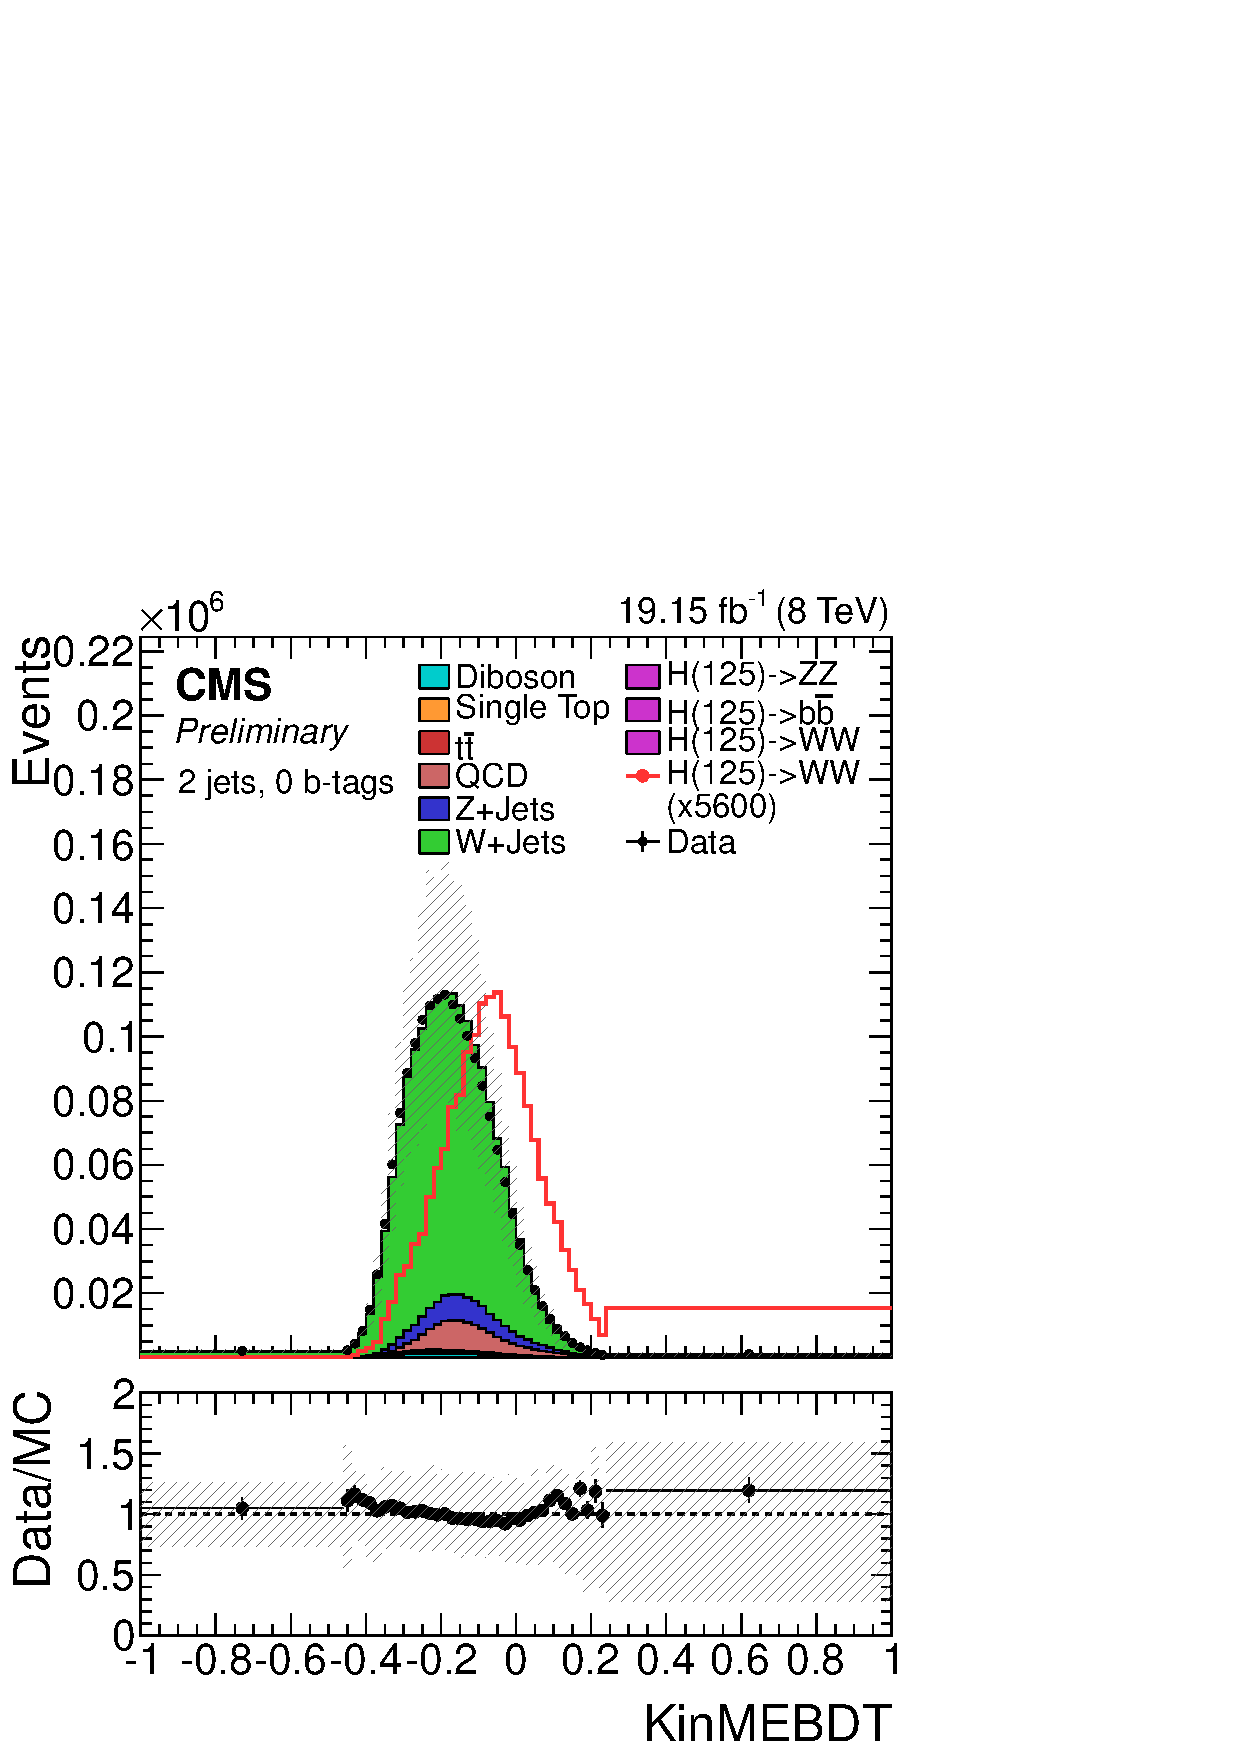
\includegraphics[width=\textwidth]{\figpath/Chapter6/KinMEBDT_jets2_electron.png}
        \caption{}
        \label{fig:KinMEBDT_jets2_electron}
    \end{subfigure}
    \begin{subfigure}[t]{0.316\textwidth}
        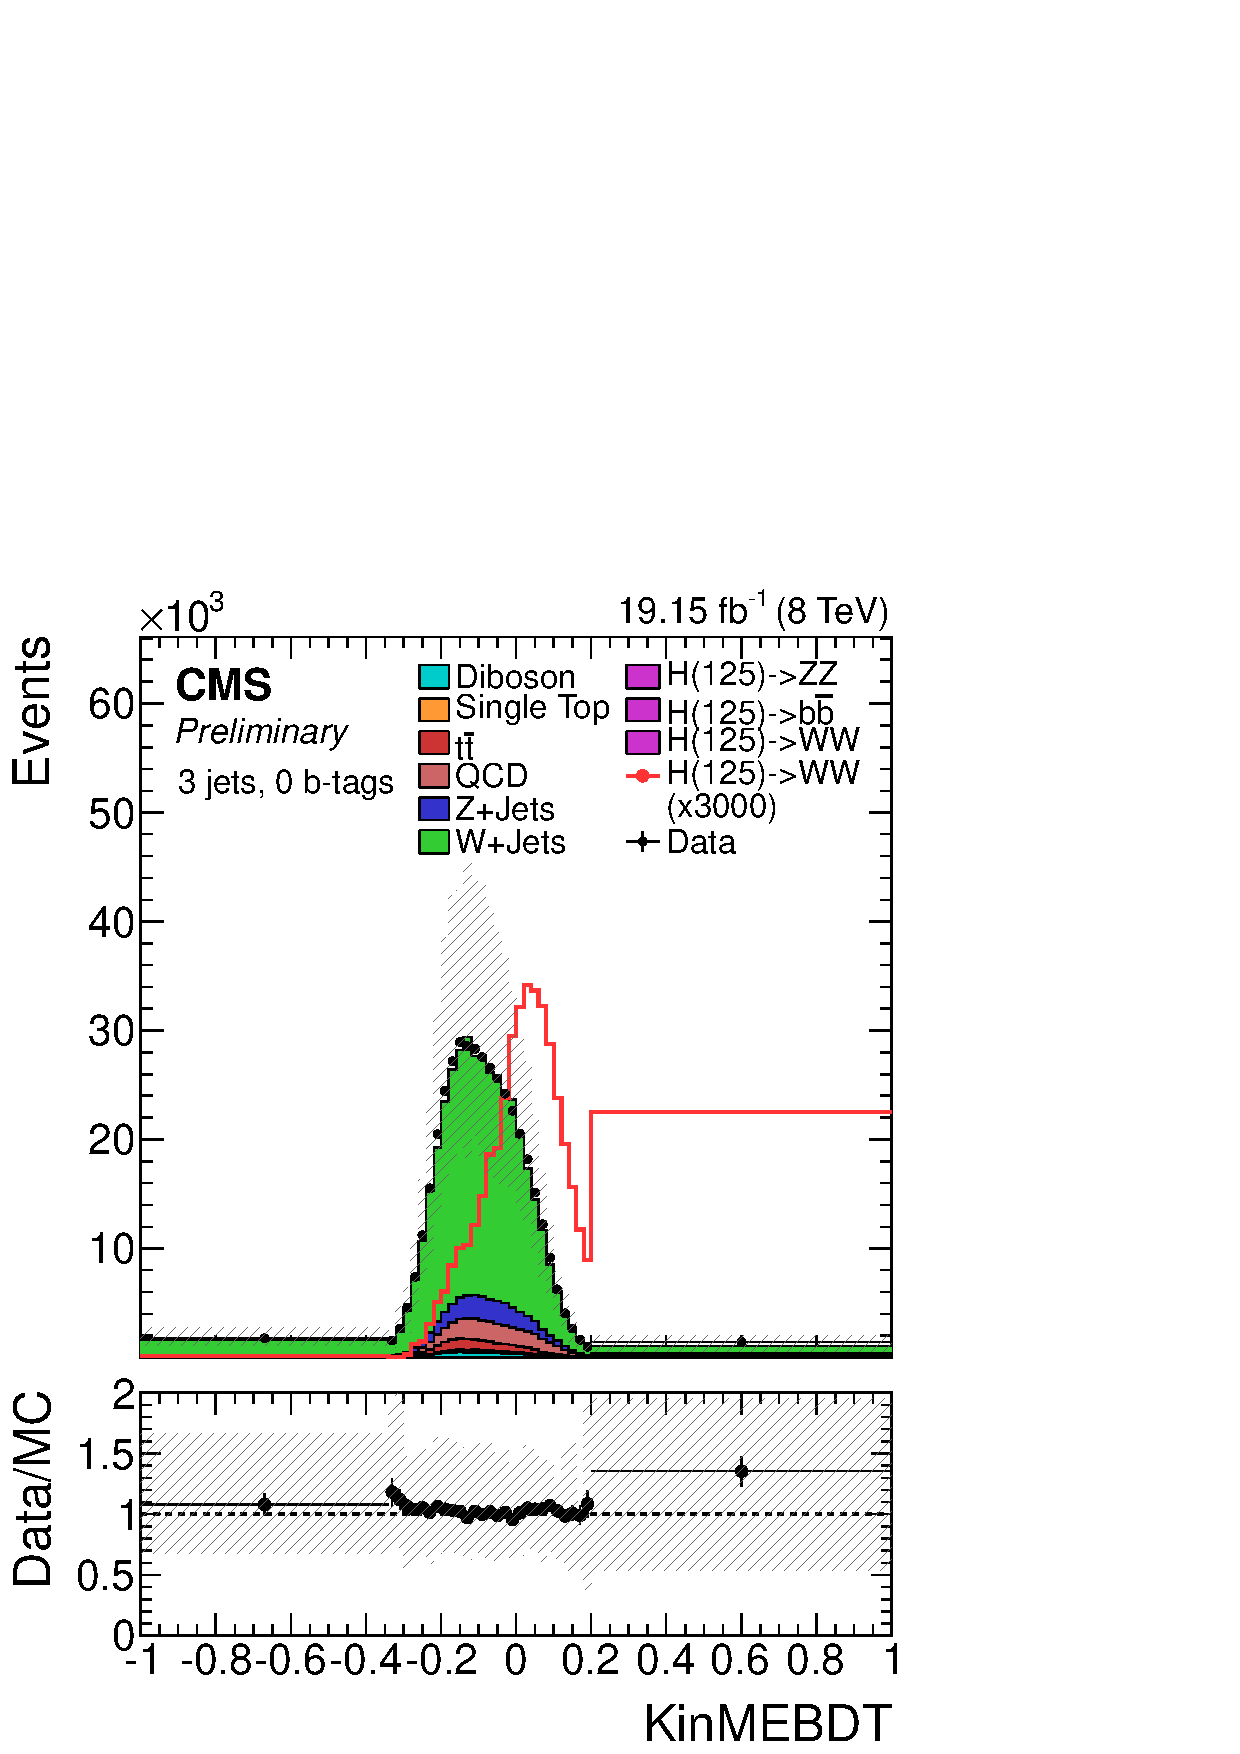
\includegraphics[width=\textwidth]{\figpath/Chapter6/KinMEBDT_jets3_electron.png}
        \caption{}
        \label{fig:KinMEBDT_jets3_electron}
    \end{subfigure}
    \begin{subfigure}[t]{0.316\textwidth}
        \includegraphics[width=\textwidth]{\figpath/Chapter6/KinMEBDT_jets4_electron.png}
        \caption{}
        \label{fig:KinMEBDT_jets4_electron}
    \end{subfigure}

    \begin{subfigure}[t]{0.316\textwidth}
        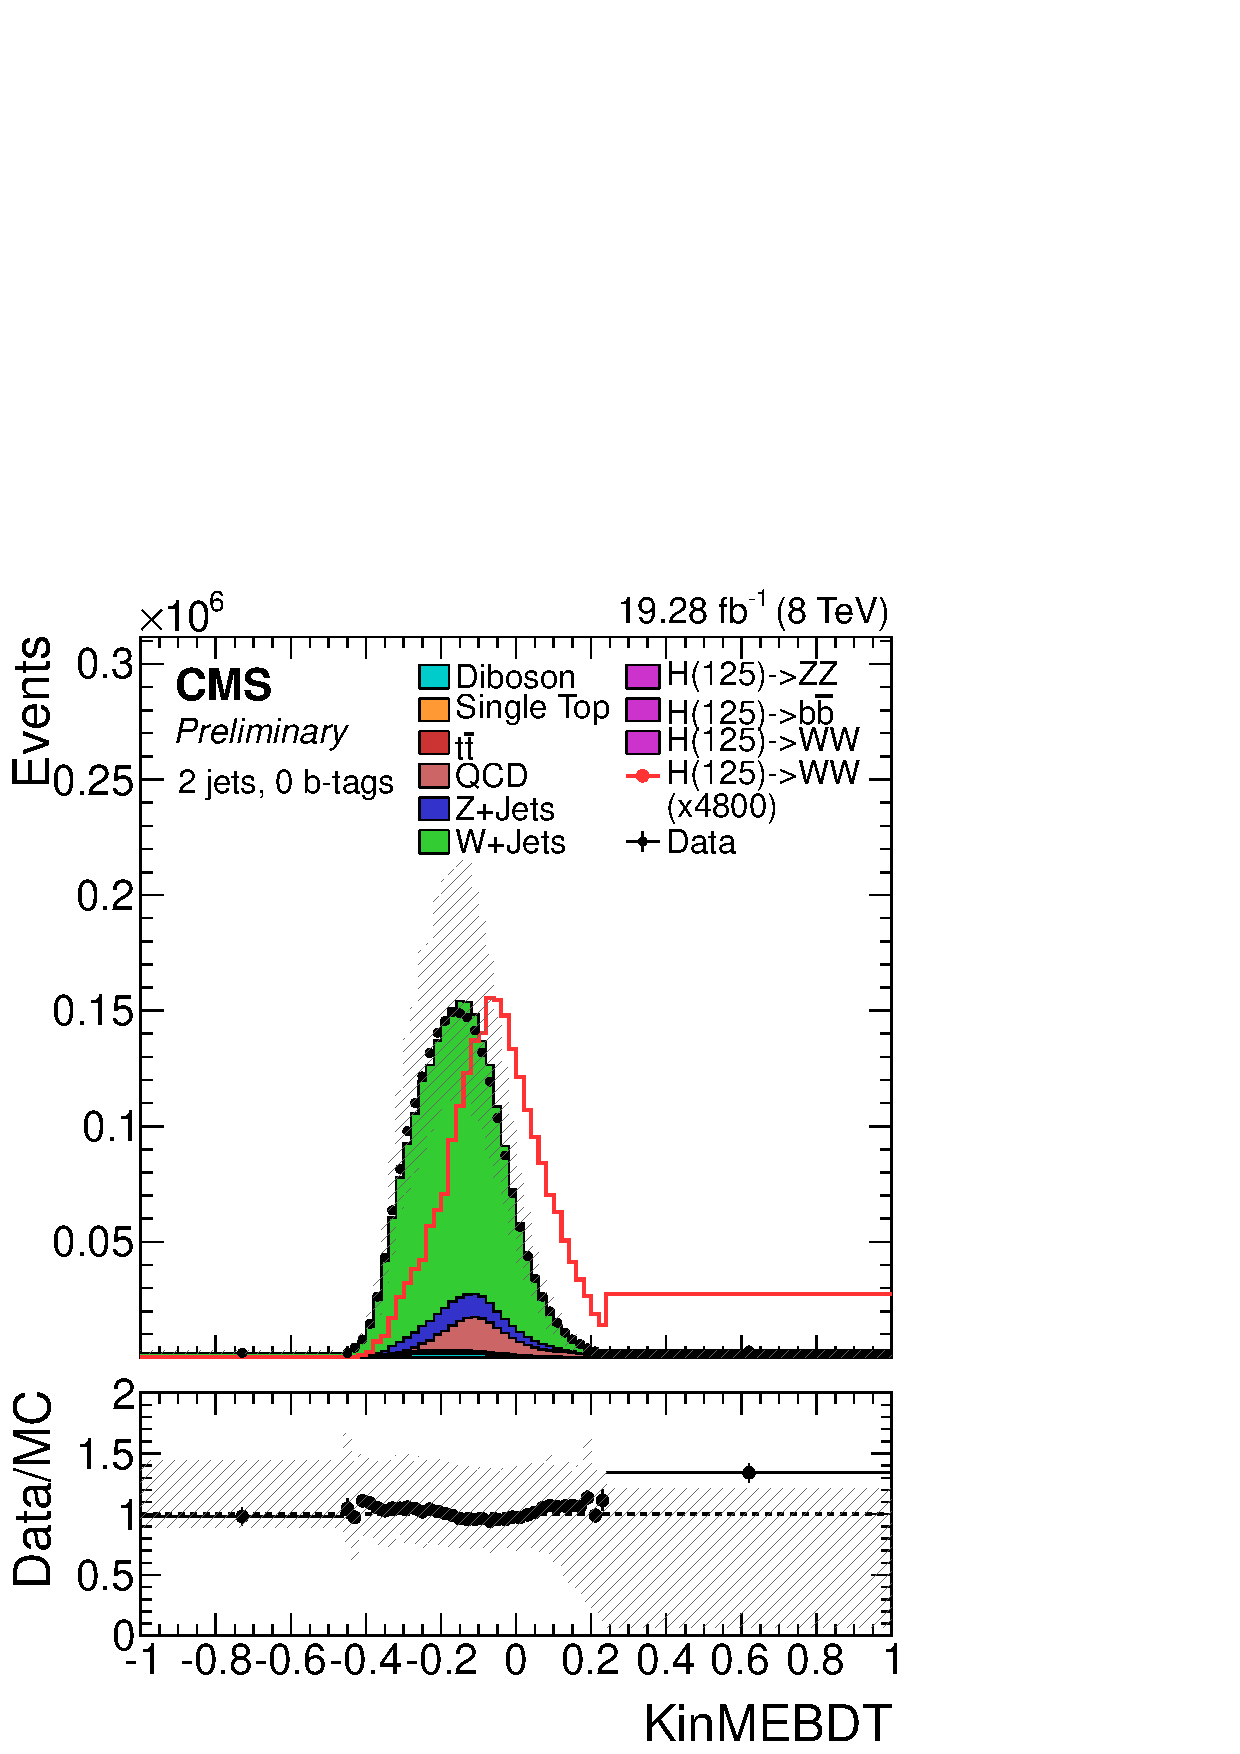
\includegraphics[width=\textwidth]{\figpath/Chapter6/KinMEBDT_jets2_muon.png}
        \caption{}
        \label{fig:KinMEBDT_jets2_muon}
    \end{subfigure}
    \begin{subfigure}[t]{0.316\textwidth}
        \includegraphics[width=\textwidth]{\figpath/Chapter6/KinMEBDT_jets3_muon.png}
        \caption{}
        \label{fig:KinMEBDT_jets3_muon}
    \end{subfigure}
    \begin{subfigure}[t]{0.316\textwidth}
        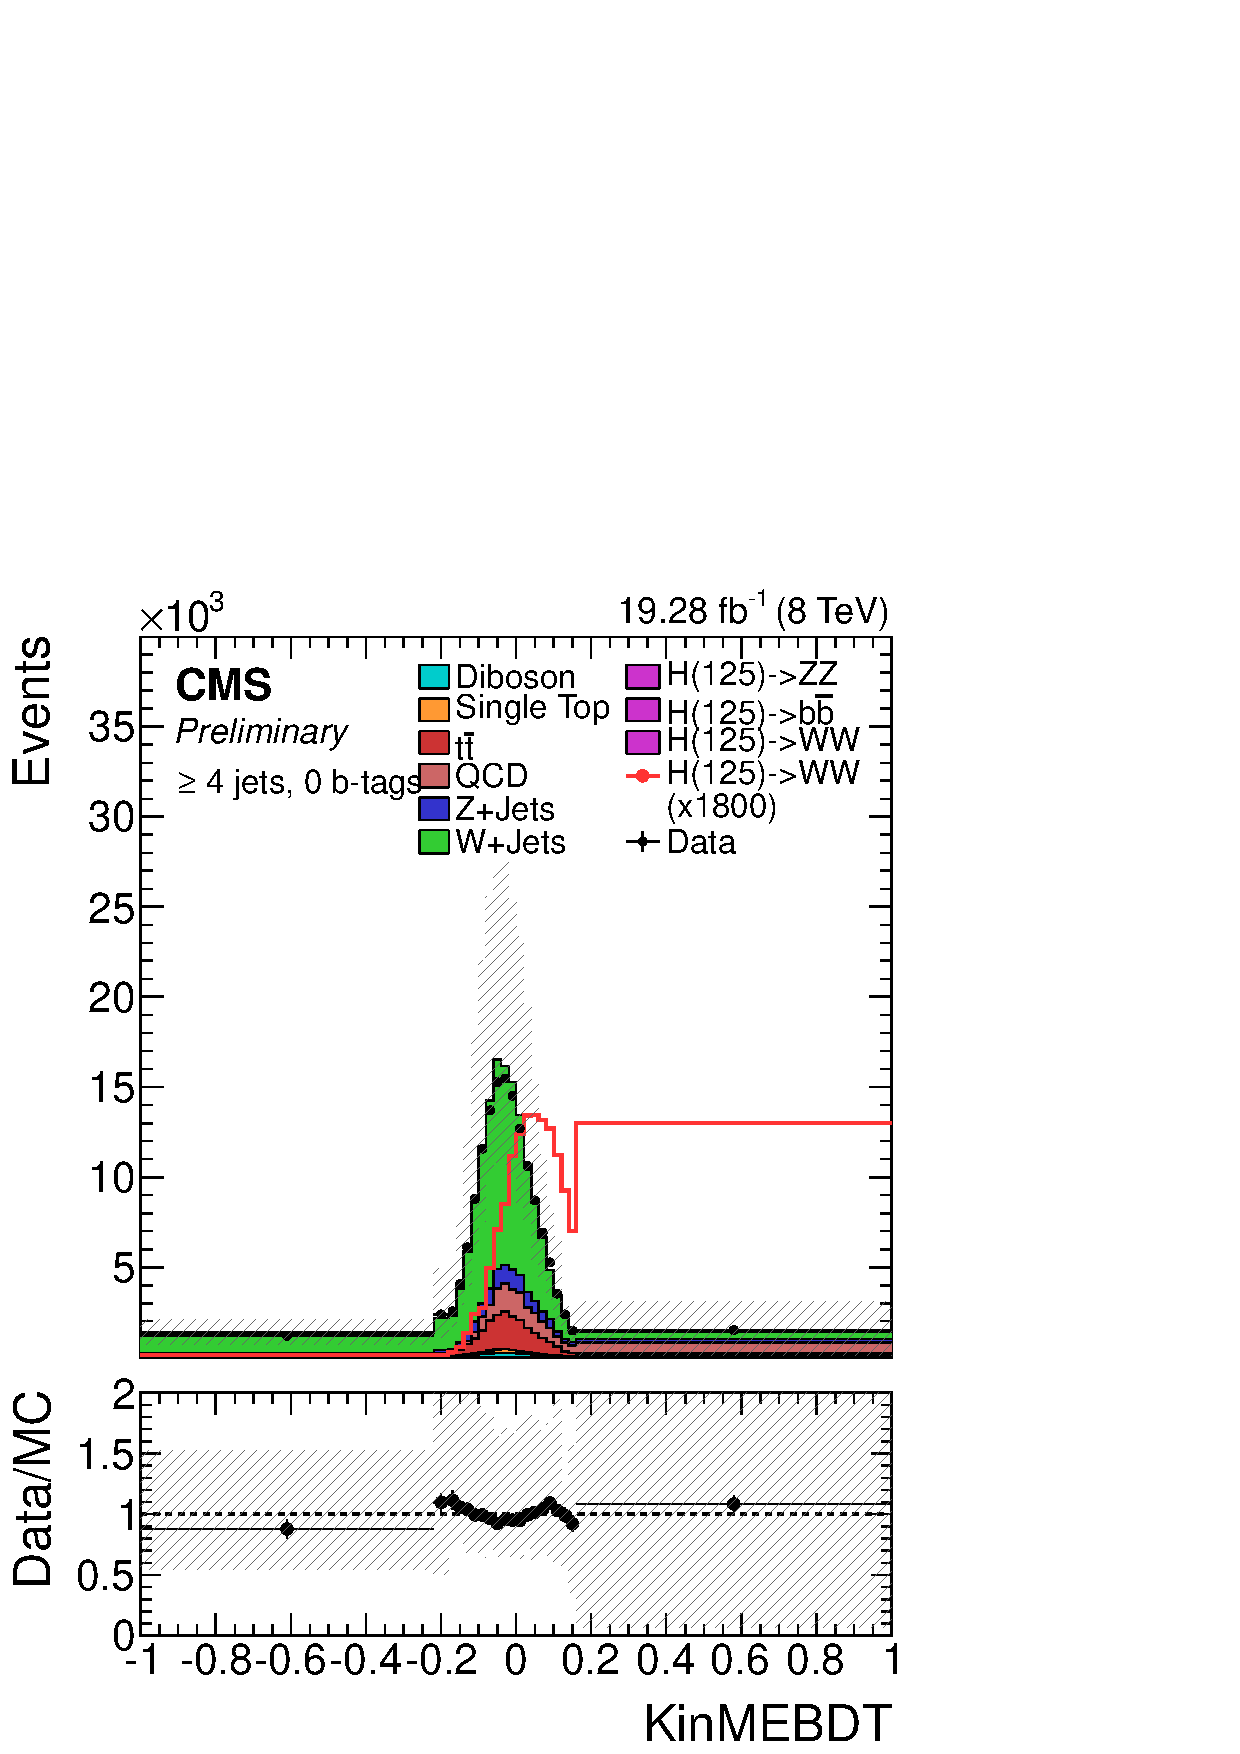
\includegraphics[width=\textwidth]{\figpath/Chapter6/KinMEBDT_jets4_muon.png}
        \caption{}
        \label{fig:KinMEBDT_jets4_muon}
    \end{subfigure}
    \caption{The KinMEBDT distribution in Monte Carlo (filled histograms) and data (black markers). The \HWW signal is shown by red line while the systematic uncertainties are shown by the hashed areas. The plots are ordered by jet bin from left to right, with the leftmost plot being the two-jet bin and the rightmost plot being the greater than or equal to four-jet bin. The top row contains the electron channel plots while the bottom rows contain the muon channel plots.}
    \label{fig:KinMEBDT_final_templates}
\end{figure}

Because no significant excess of signal events was observed, the best we can do is set an upper limit on the production cross sections of \HWWlvjj.
The results are reported as an upper bound on $\sigma/\sigma_{\text{SM}}$ at the 95\% confidence level (CL), made by using the modified-frequentist limit setting method with the CL\textsubscript{S} test statistic~\cite{Read:presentation,Junk,LHC-HCG}.
Although it is more rigorous to use the toy-based frequentist limit setting procedures, these methods are known to take an exceedingly long time to converge.
However, when not in a low statistics regime, the toy-based methods and the asymptotic approximation return roughly equivalent answers.
Therefore, we used the asymptotic approximation as we do indeed have copious amounts of background and data in our templates.
The computations were done using the Higgs Combine Tool~\cite{HiggsCombineTwiki}, which is a RooStats~\cite{Schott:2012zb} based limit setting package.
Appendix~\ref{appendix:limit_setting} contains a more detailed discussion on the computation of the CL\textsubscript{S} limits.
The expected and observed upper limits on $\sigma/\sigma_{\text{SM}}$ are shown in fig.~\ref{fig:limits_withSys_muon}, with the actual values listed in table~\ref{tab:95percent_upper_confidence_levels}.

\begin{comment}
Rishi:
The p-value of the excess at 125 GeV is 3.2σ.

To quantify, how probable the observed excess of events is above the background fluctuations the combined p-value is computed for the best-fit Higgs mass of 124.7GeV with a statistical significance of 5.65σ
\end{comment}

\begin{figure}[!hbt]
    \centering
    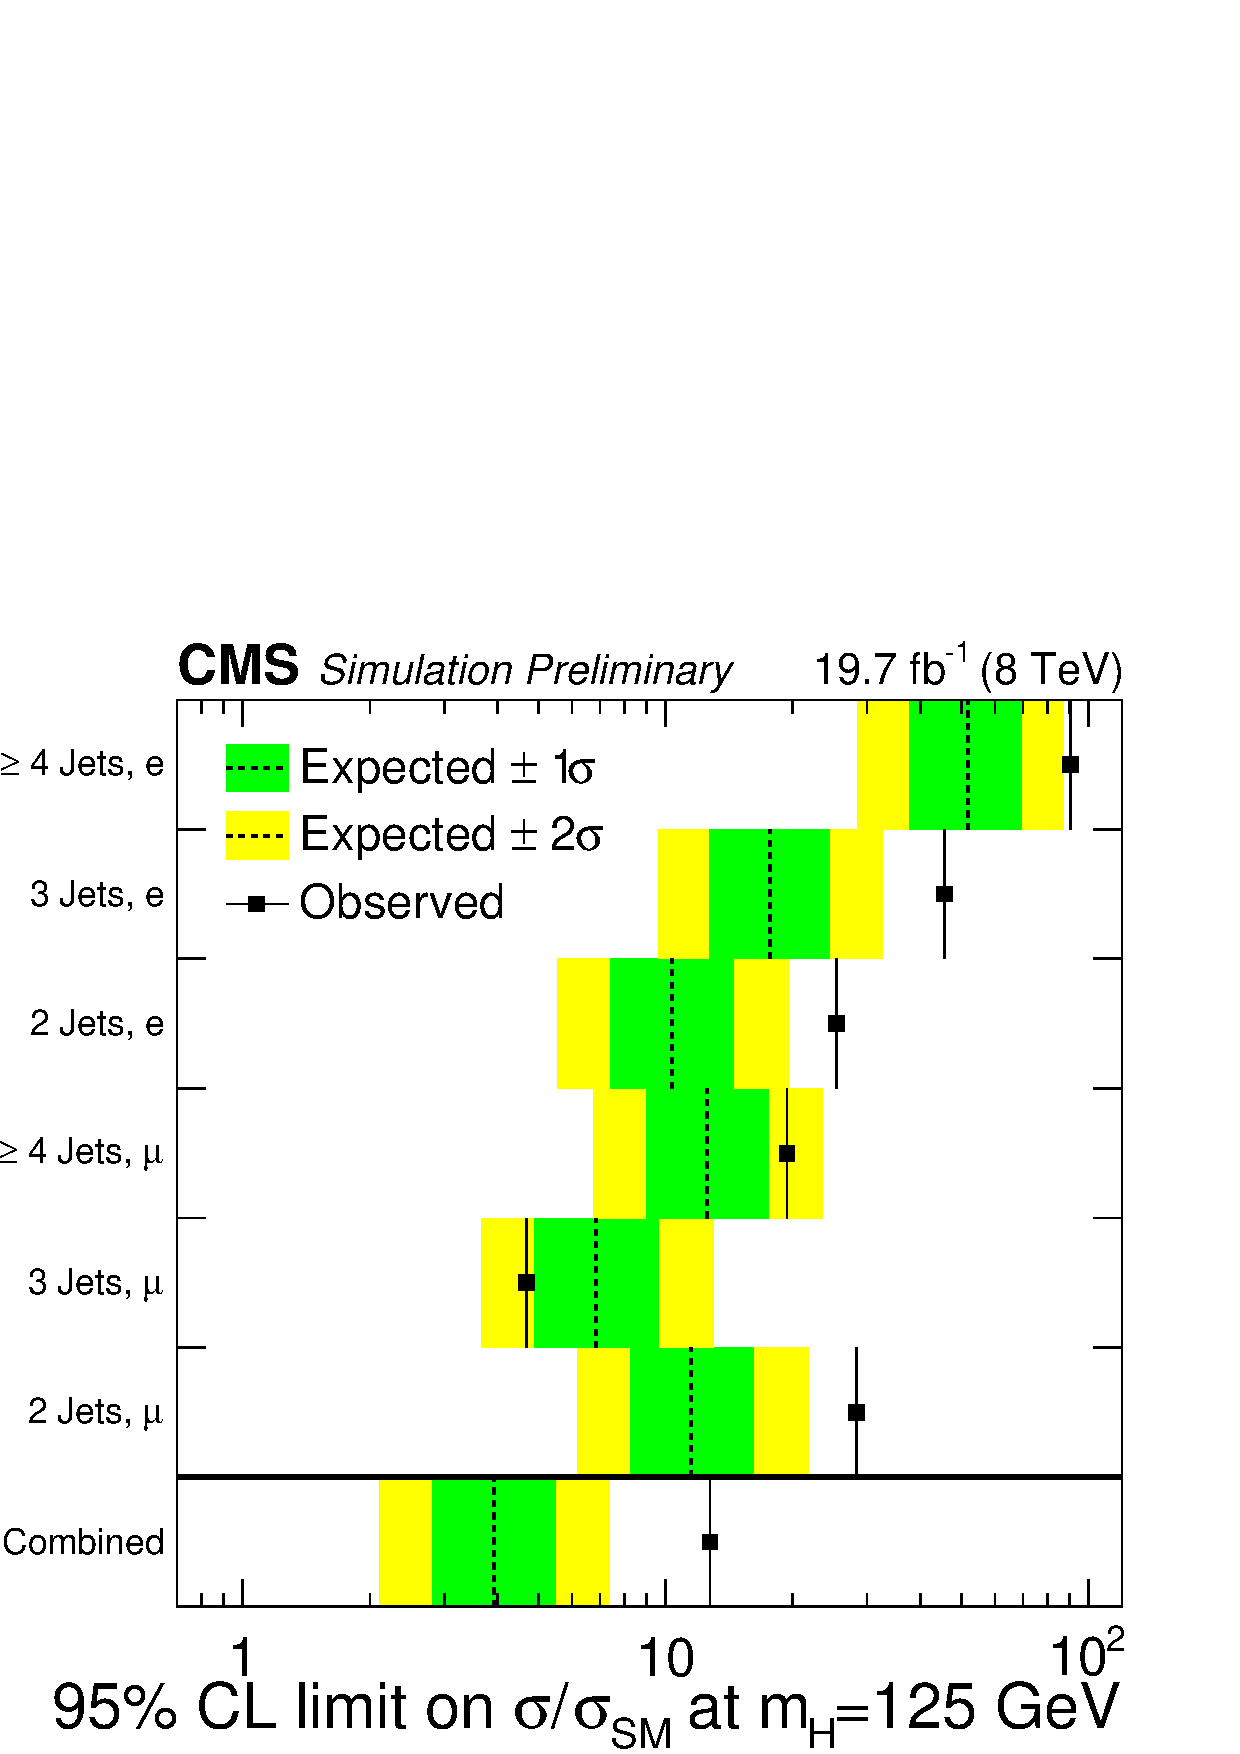
\includegraphics[width=0.95\textwidth]{\figpath/Chapter6/2017_11_13_combinedSM_KinMEBDT.pdf}
    \caption{Median expected and observed 95\% upper confidence level on the cross-section ratio to the expected Standard Model Higgs cross-section ($\mu$) for only the muon channel. The green and yellow uncertainty bands represent the 68\% and 95\% CL intervals on the expected limit, respectively. The values were found using the Asymptotic CL\textsubscript{S} approximation.}
    \label{fig:limits_withSys_muon}
\end{figure}

\begin{table}[htbp]
\centering
\begin{tabular}{lrr} \hline
Category                            & Observed & Expected               \\
\hline\\[-2.45ex]
$\geqslant$4 Jets (\Pe)             & $90.6$   & $51.9_{-14.1}^{+17.6}$ \\
3 Jets (\Pe)                        & $45.6$   & $17.7_{-5.0}^{+6.7}$   \\
2 Jets (\Pe)                        & $25.4$   & $10.3_{-2.9}^{+4.2}$   \\
$\geqslant$4 Jets (\Pmu)            & $19.4$   & $12.6_{-3.6}^{+5.0}$   \\
3 Jets (\Pmu)                       & $4.7$    & $6.8_{-1.9}^{+2.8}$    \\
2 Jets (\Pmu)                       & $28.2$   & $11.5_{-3.3}^{+4.6}$   \\
\hline\\[-2.45ex]
%2 Jets (Combined Lepton)            &          & $7.2_{-5.2}^{+10.0}$  \\
%3 Jets (Combined Lepton)            &          & $4.7_{-3.4}^{+6.6}$   \\
%$\geqslant$4 Jets (Combined Lepton) &          & $8.2_{-5.8}^{+11.4}$  \\
%\hline\\[-2.45ex]
%Combined Jets (\Pe)                 &          & $4.0_{-1.1}^{+1.6}$   \\
%Combined Jets (\Pmu)                & $4.1$    & $5.4_{-1.5}^{+2.2}$   \\
%\hline\\[-2.45ex]
Combined                            & 12.7      & $3.9_{-1.1}^{+1.6}$   \\
%Significance: 4.08718
%       (p-value = 2.1832e-05)
\hline
\end{tabular}
\caption{Observed and median expected and 95\% CLs upper limits on $\mu$ calculated with the Asymptotic CL\textsubscript{S} method. The $\pm1\sigma$ confidence interval is quoted for the expected limits.}
\label{tab:95percent_upper_confidence_levels}
\end{table}
%The next line is the format for inserting new sections.
%Replace the name "newsection"  with the name of your
%new section file.
%\include{data/newsection}

%fix spacing in bibliography, if any...
%%%%%%%%%%%%%%%%%%%%%%%%%%%%%%%%%%%%%%%%%%%%%%%%%%%%%%%%%%%%%
\let\oldbibitem\bibitem
\renewcommand{\bibitem}{\setlength{\itemsep}{0pt}\oldbibitem}
%%%%%%%%%%%%%%%%%%%%%%%%%%%%%%%%%%%%%%%%%%%%%%%%%%%%%%%%%%%%%%%
%The bibliography style declared is the IEEE format. If
%you require a different style, see the document
%bibstyles.pdf included in this package. This file,
%hosted by the University of Vienna, shows several
%bibliography styles and examples of in-text citation
%and a references page.
\bibliographystyle{ieeetr}

\phantomsection
\addcontentsline{toc}{chapter}{REFERENCES}

\renewcommand{\bibname}{{\normalsize\rm REFERENCES}}

%This file is a .bib database that contains the sources.
%This removes the dependency on the previous file
%bibliography.tex.
\bibliography{data/myReference}




%This next line includes appendices. The file
%appendix.tex contains commands pointing to
%the appendix files; be sure to change these
%pointers if you end up changing the filenames.
%Leave this commented if you will not need
%appendix material.
%!TEX root = ../TAMUTemplate.tex
%%%%%%%%%%%%%%%%%%%%%%%%%%%%%%%%%%%%%%%%%%%%%%%%%%%
%
%  New template code for TAMU Theses and Dissertations starting Fall 2016.  
%
%
%  Author: Sean Zachary Roberson 
%	 Version 3.16.09
%  Last updated 9/12/2016
%
%%%%%%%%%%%%%%%%%%%%%%%%%%%%%%%%%%%%%%%%%%%%%%%%%%%

\begin{appendices}
\titleformat{\chapter}{\centering\normalsize}{APPENDIX \thechapter}{0em}{\vskip .5\baselineskip\centering}
\renewcommand{\appendixname}{APPENDIX}

%!TEX root = ../TAMUTemplate.tex
%%%%%%%%%%%%%%%%%%%%%%%%%%%%%%%%%%%%%%%%%%%%%%%%%%%
%
%  New template code for TAMU Theses and Dissertations starting Fall 2016.
%
%
%  Author: Sean Zachary Roberson 
%	 Version 3.16.09
%  Last updated 9/12/2016
%
%%%%%%%%%%%%%%%%%%%%%%%%%%%%%%%%%%%%%%%%%%%%%%%%%%%

%%%%%%%%%%%%%%%%%%%%%%%%%%%%%%%%%%%%%%%%%%%%%%%%%%%%%%%%%%%%%%%%%%%%%%
%%                           APPENDIX A
%%%%%%%%%%%%%%%%%%%%%%%%%%%%%%%%%%%%%%%%%%%%%%%%%%%%%%%%%%%%%%%%%%%%%

\phantomsection

\chapter{\uppercase{History of the Standard Model}}
\label{appendix:standard_model_history}
%!TEX root = ../TAMUTemplate.tex
%%%%%%%%%%%%%%%%%%%%%%%%%%%%%%%%%%%%%%%%%%%%%%%%%%%
%
%  New template code for TAMU Theses and Dissertations starting Fall 2016.
%
%
%  Author: Sean Zachary Roberson 
%	 Version 3.16.09
%  Last updated 9/12/2016
%
%%%%%%%%%%%%%%%%%%%%%%%%%%%%%%%%%%%%%%%%%%%%%%%%%%%

%%%%%%%%%%%%%%%%%%%%%%%%%%%%%%%%%%%%%%%%%%%%%%%%%%%%%%%%%%%%%%%%%%%%%%
%%                           APPENDIX B 
%%%%%%%%%%%%%%%%%%%%%%%%%%%%%%%%%%%%%%%%%%%%%%%%%%%%%%%%%%%%%%%%%%%%%

\chapter{\uppercase{Boosted Decision Tree}}

\section{Inputs}
\section{Outputs}
\section{Correlations}
\section{Architecture Variables}


%!TEX root = ../TAMUTemplate.tex
%%%%%%%%%%%%%%%%%%%%%%%%%%%%%%%%%%%%%%%%%%%%%%%%%%%
%
%  New template code for TAMU Theses and Dissertations starting Fall 2016.
%
%
%  Author: Sean Zachary Roberson 
%	 Version 3.16.09
%  Last updated 9/12/2016
%
%%%%%%%%%%%%%%%%%%%%%%%%%%%%%%%%%%%%%%%%%%%%%%%%%%%

%%%%%%%%%%%%%%%%%%%%%%%%%%%%%%%%%%%%%%%%%%%%%%%%%%%%%%%%%%%%%%%%%%%%%%
%%                           APPENDIX C
%%%%%%%%%%%%%%%%%%%%%%%%%%%%%%%%%%%%%%%%%%%%%%%%%%%%%%%%%%%%%%%%%%%%%

\phantomsection

\chapter{\uppercase{\VETslash Performance and Corrections}}
\label{appendix:MET}

\section{Type-0 \VETslash Correction}
Pileup interactions typically produce visible particles, with only a few processes, like neutrinos from Kaon decays, producing invisible particles.
If CMS were able to perfectly measure all of the visible particles then pileup would have little effect on the \VETslash reconstruction.
However, as discussed in section~\ref{sec:MET}, the \VETslash reconstruction does degrade as the number of pileup interactions increases.
The type-0 correction is an attempt to remove this pileup effect for the \VETslash calculated using PF candidates, as opposed to calorimeter towers or tracks.

In essence, the type-0 correction is an application of CHS (see~\ref{sec:jets} for a discussion of CHS), but also removes a portion of the \VETslash estimated to come from neutral pileup. The neutral pileup estimate is necessary because removing only charged particles might cause the \VETslash to move further from its true value. In this section the pileup particles will be broken up as being neutral (neuPU) or charges (chPU). Furthermore, the correction makes three assumptions about the pileup particles as spelled out in equation~\ref{eq:MET_type0_assumptions}. The first assumption is that the sum of \pt for the neutral and charged components of the \VETslash due to pileup are equal and opposite. At the truth level this cancellation is very nearly exact. The part of~\ref{eq:MET_type0_assumptions} says that the charged particles can be measured exactly, which is also a good assumption for low \ptvec tracks. The last assumption says that the direction of the neutral pileup can be measured exactly, but that the energy is off by the same amount for each particle. The directionality is measured using the position of the calorimeter cells, but the energy measurement calibration was done using high \ptvec particles so that the system systematically mismeasures low \ptvec particles.
\begin{equation}
\begin{aligned}
	\label{eq:MET_type0_assumptions}
\sum_{i \in \textrm{neuPU}}\ptvecsubsup{i}{true}+\sum_{i \in \textrm{chPU}}\ptvecsubsup{i}{true}=0 \\
\sum_{i \in \textrm{chPU}}\ptvecsubsup{i}{true}=\sum_{i \in \textrm{chPU}}\ptvecsub{i} \\
\sum_{i \in \textrm{neuPU}}\ptvecsub{i}=R^{0}\sum_{i \in \textrm{neuPU}}\ptvecsub{i}
\end{aligned}
\end{equation}
The assumptions can then be combined into equation~\ref{eq:MET_type0_replace}.
\begin{equation}
\begin{aligned}
	\label{eq:MET_type0_replace}
\sum_{i \in \textrm{neuPU}}\ptvecsub{i}=-R^{0}\sum_{i \in \textrm{chPU}}\ptvecsub{i}
\end{aligned}
\end{equation}

The raw \VETslash components can be broken up as coming from either the hard scatter (HS) vertex or from pileup (PU) interactions. The pileup can then be further boken down into the neutral and charged components as previously specified. This categorization is shown in equation~\ref{eq:MET_type0_raw}.
\begin{equation}
\begin{aligned}
	\label{eq:MET_type0_raw}
\VETslashraw={}&-\sum_{i \in \textrm{HS}}\ptvecsub{i}-\sum_{i \in \textrm{PU}}\ptvecsub{i} \\
={}&-\sum_{i \in \textrm{HS}}\ptvecsub{i}-\sum_{i \in \textrm{neuPU}}\ptvecsub{i}-\sum_{i \in \textrm{chPU}}\ptvecsub{i}
\end{aligned}
\end{equation}
CHS is able to remove the third sum, but is not able to separate the first and second sums.

The type-0 corrections is the estimate of the neutral pileup shown in equation~\ref{eq:MET_type0_replace} plus the sum over the charged particles from pileup.
\begin{equation}
	\label{eq:MET_type0_correction}
\vec{C}_{\mathrm{T}}^{Type-0}=\left(1-R^{0}\right)\sum_{i \in \mathrm{chPU}}\ptvecsub{i}
\end{equation}
This corrections added to the raw \VETslash yields the type-0 corrected \VETslash. To also propogate the JEC to the pileup corrected \VETslash one can add type-1 correction to the type-0 corrected \VETslash. This process can be seen in equation~\ref{eq:MET_type0}. 
\begin{equation}
\begin{aligned}
	\label{eq:MET_type0}
\VETslashsup{Type-0\hspace{-0.22em}}\hspace{0.37em}={}&\VETslashraw+\vec{C}_{\mathrm{T}}^{\mathrm{Type-0}} \\
\VETslashsupwide{Type-0-1}={}&\VETslashsup{Type-0\hspace{-0.22em}}\hspace{0.37em}+\vec{C}_{\mathrm{T}}^{\mathrm{Type-1}}
\end{aligned}
\end{equation}



\section{\VETslash Filters}
Besides interesting physics processes, high values of \ETslash can be caused by cosmic rays, detector noise, and particles from the beam-halo.
In addition to the previous corrections used to make sure the \VETslash is reconstructed correctly, CMS has also developed several algorithms for identifying and removing sources of fake \VETslash.
False \VETslash is a problem because is causes a discrepancy between the data and MC, where the sources of fake \VETslash are not explicitly simulated.
After several of these filters are used this agreement will typically improve.

%!TEX root = ../TAMUTemplate.tex
%%%%%%%%%%%%%%%%%%%%%%%%%%%%%%%%%%%%%%%%%%%%%%%%%%%
%
%  New template code for TAMU Theses and Dissertations starting Fall 2016.
%
%
%  Author: Sean Zachary Roberson 
%	 Version 3.16.09
%  Last updated 9/12/2016
%
%%%%%%%%%%%%%%%%%%%%%%%%%%%%%%%%%%%%%%%%%%%%%%%%%%%

%%%%%%%%%%%%%%%%%%%%%%%%%%%%%%%%%%%%%%%%%%%%%%%%%%%%%%%%%%%%%%%%%%%%%%
%%                           APPENDIX D 
%%%%%%%%%%%%%%%%%%%%%%%%%%%%%%%%%%%%%%%%%%%%%%%%%%%%%%%%%%%%%%%%%%%%%

\chapter{\texorpdfstring{\uppercase{Boosted Decision Trees}}{Boosted Decision Trees}}

\section{Inputs}
\label{appendix:BDT_Inputs}

\begin{figure}[!hbt]
    \centering
    \begin{subfigure}[t]{0.93\textwidth}
        \includegraphics[width=\textwidth]{\figpath/Chapter5/BDT_Performance_Plots/BDT_InputVars_2j0B_p1.png}
        \caption{}
        \label{fig:BDT_InputVars_2j0B_p1}
    \end{subfigure}

    \begin{subfigure}[t]{0.93\textwidth}
        \includegraphics[width=\textwidth]{\figpath/Chapter5/BDT_Performance_Plots/BDT_InputVars_2j0B_p2.png}
        \caption{}
        \label{fig:BDT_InputVars_2j0B_p2}
    \end{subfigure}
    \caption{Inputs used to train the BDTs with kinematic variables in the 2 jets bin.}
    \label{fig:BDT_InputVars_2j0B}
\end{figure}

\begin{figure}[!hbt]
    \centering
    \begin{subfigure}[t]{0.93\textwidth}
        \includegraphics[width=\textwidth]{\figpath/Chapter5/BDT_Performance_Plots/BDT_InputVars_3j0B_p1.png}
        \caption{}
        \label{fig:BDT_InputVars_3j0B_p1}
    \end{subfigure}

    \begin{subfigure}[t]{0.93\textwidth}
        \includegraphics[width=\textwidth]{\figpath/Chapter5/BDT_Performance_Plots/BDT_InputVars_3j0B_p2.png}
        \caption{}
        \label{fig:BDT_InputVars_3j0B_p2}
    \end{subfigure}

    \begin{subfigure}[t]{0.93\textwidth}
        \includegraphics[trim={0 7.3cm 0 0},clip,width=\textwidth]{\figpath/Chapter5/BDT_Performance_Plots/BDT_InputVars_3j0B_p3.png}
        \caption{}
        \label{fig:BDT_InputVars_3j0B_p3}
    \end{subfigure}
    \caption{Inputs used to train the BDTs with kinematic variables in the 3 jets bin.}
    \label{fig:BDT_InputVars_3j0B}
\end{figure}

\begin{figure}[!hbt]
    \centering
    \begin{subfigure}[t]{0.93\textwidth}
        \includegraphics[width=\textwidth]{\figpath/Chapter5/BDT_Performance_Plots/BDT_InputVars_4j0B_p1.png}
        \caption{}
        \label{fig:BDT_InputVars_4j0B_p1}
    \end{subfigure}

    \begin{subfigure}[t]{0.93\textwidth}
        \includegraphics[width=\textwidth]{\figpath/Chapter5/BDT_Performance_Plots/BDT_InputVars_4j0B_p2.png}
        \caption{}
        \label{fig:BDT_InputVars_4j0B_p2}
    \end{subfigure}
    \caption{Inputs used to train the BDTs with kinematic variables in the $\geqslant$4 jets bin.}
    \label{fig:BDT_InputVars_4j0B}
\end{figure}
\clearpage
















\section{Outputs}
\label{appendix:BDT_Outputs}
\begin{figure}[!hbt]
    \centering
    \begin{subfigure}[t]{0.317\textwidth}
        \includegraphics[width=\textwidth]{\figpath/Chapter5/BDT_Performance_Plots/BDT_Response_2j0B.png}
        \caption{}
        \label{fig:BDT_Response_2j0B_TMVA}
    \end{subfigure}
    \begin{subfigure}[t]{0.317\textwidth}
        \includegraphics[width=\textwidth]{\figpath/Appendix5/jets2/electron/KinBDT_electron.eps}
        \caption{}
        \label{fig:KinBDT_jets2_electron_noSys}
    \end{subfigure}
    \begin{subfigure}[t]{0.317\textwidth}
        \includegraphics[width=\textwidth]{\figpath/Appendix5/jets2/muon/KinBDT_muon.eps}
        \caption{}
        \label{fig:KinBDT_jets2_muon_noSys}
    \end{subfigure}
    \caption{(a) The BDT response plot from TMVA for the training with only kinematic variables in the 2 jet bin for the combined lepton channel. Validation plot for the BDT in the 2 jet bin for the (b) electron and (c) muon channels. Only statistical uncertainties are shown in the validation plots.}
    \label{fig:KinBDT_Comparison_jets2}
\end{figure}

\begin{figure}[!hbt]
    \centering
    \begin{subfigure}[t]{0.317\textwidth}
        \includegraphics[width=\textwidth]{\figpath/Chapter5/BDT_Performance_Plots/BDT_Response_3j0B.png}
        \caption{}
        \label{fig:BDT_Response_3j0B_TMVA}
    \end{subfigure}
    \begin{subfigure}[t]{0.317\textwidth}
        \includegraphics[width=\textwidth]{\figpath/Appendix5/jets3/electron/KinBDT_electron.eps}
        \caption{}
        \label{fig:KinBDT_jets3_electron_noSys}
    \end{subfigure}
    \begin{subfigure}[t]{0.317\textwidth}
        \includegraphics[width=\textwidth]{\figpath/Appendix5/jets3/muon/KinBDT_muon.eps}
        \caption{}
        \label{fig:KinBDT_jets3_muon_noSys}
    \end{subfigure}
    \caption{(a) The BDT response plot from TMVA for the training with only kinematic variables in the 3 jet bin for the combined lepton channel. Validation plot for the BDT in the 3 jet bin for the (b) electron and (c) muon channels. Only statistical uncertainties are shown in the validation plots.}
    \label{fig:KinBDT_Comparison_jets3}
\end{figure}

\begin{figure}[!hbt]
    \centering
    \begin{subfigure}[t]{0.317\textwidth}
        \includegraphics[width=\textwidth]{\figpath/Chapter5/BDT_Performance_Plots/BDT_Response_4j0B.png}
        \caption{}
        \label{fig:BDT_Response_4j0B_TMVA}
    \end{subfigure}
    \begin{subfigure}[t]{0.317\textwidth}
        \includegraphics[width=\textwidth]{\figpath/Appendix5/jets4/electron/KinBDT_electron.eps}
        \caption{}
        \label{fig:KinBDT_jets4_electron_noSys}
    \end{subfigure}
    \begin{subfigure}[t]{0.317\textwidth}
        \includegraphics[width=\textwidth]{\figpath/Appendix5/jets4/muon/KinBDT_muon.eps}
        \caption{}
        \label{fig:KinBDT_jets4_muon_noSys}
    \end{subfigure}
    \caption{(a) The BDT response plot from TMVA for the training with only kinematic variables in the $\geqslant$4 jet bin for the combined lepton channel. Validation plot for the BDT in the $\geqslant$4 jet bin for the (b) electron and (c) muon channels. Only statistical uncertainties are shown in the validation plots.}
    \label{fig:KinBDT_Comparison_jets4}
\end{figure}

\begin{figure}[!hbt]
    \centering
    \begin{subfigure}[t]{0.317\textwidth}
        \includegraphics[width=\textwidth]{\figpath/Appendix5/jets2/2015_07_17_TMVA_output_jets2_eq0tag_both_HToWW_WJets_allEvtProbs_0KinVar/mva_BDT.pdf}
        \caption{}
        \label{fig:MEBDT_Response_2j0B_TMVA}
    \end{subfigure}
    \begin{subfigure}[t]{0.317\textwidth}
        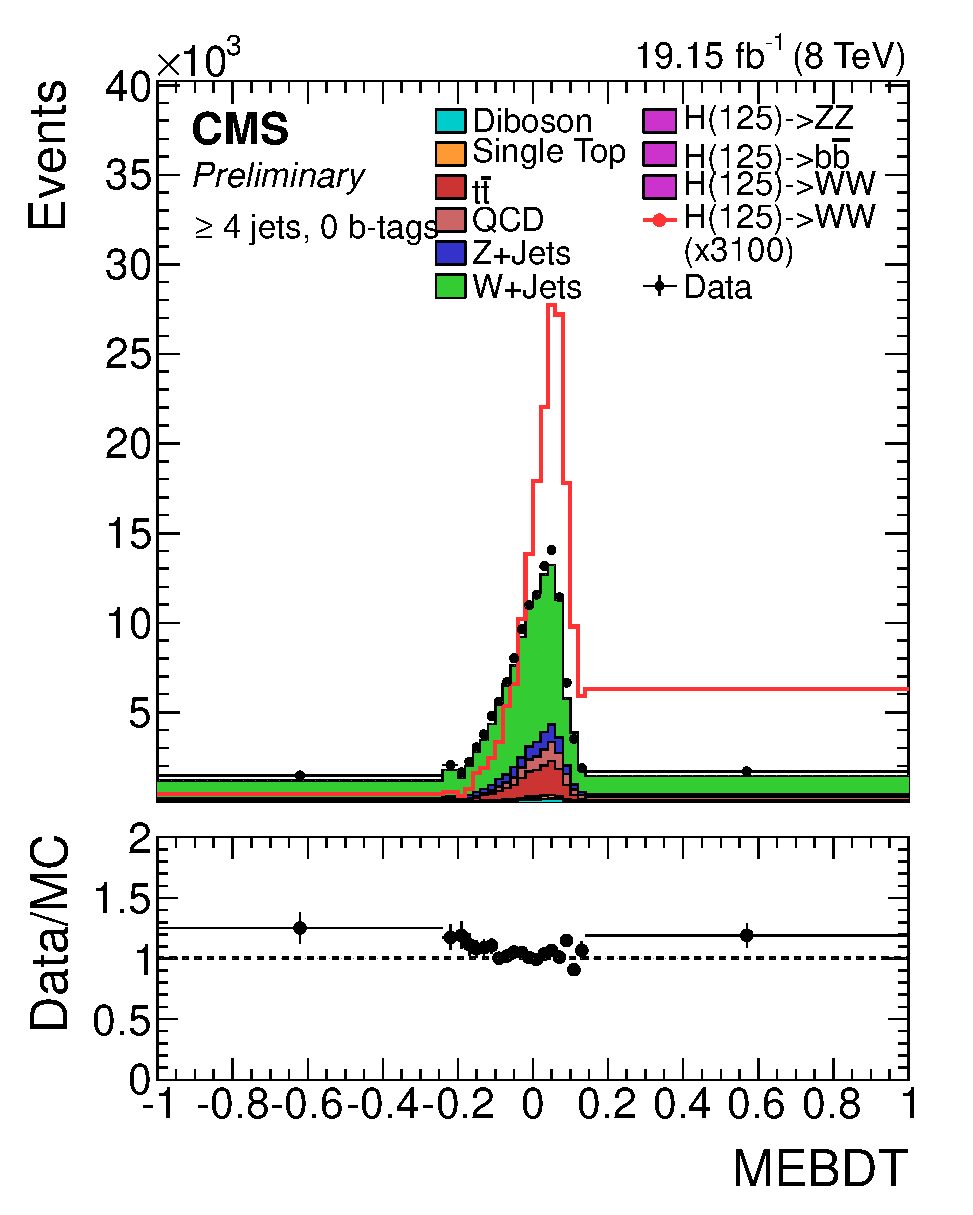
\includegraphics[width=\textwidth]{\figpath/Appendix5/jets2/electron/MEBDT_electron.eps}
        \caption{}
        \label{fig:MEBDT_jets2_electron_noSys}
    \end{subfigure}
    \begin{subfigure}[t]{0.317\textwidth}
        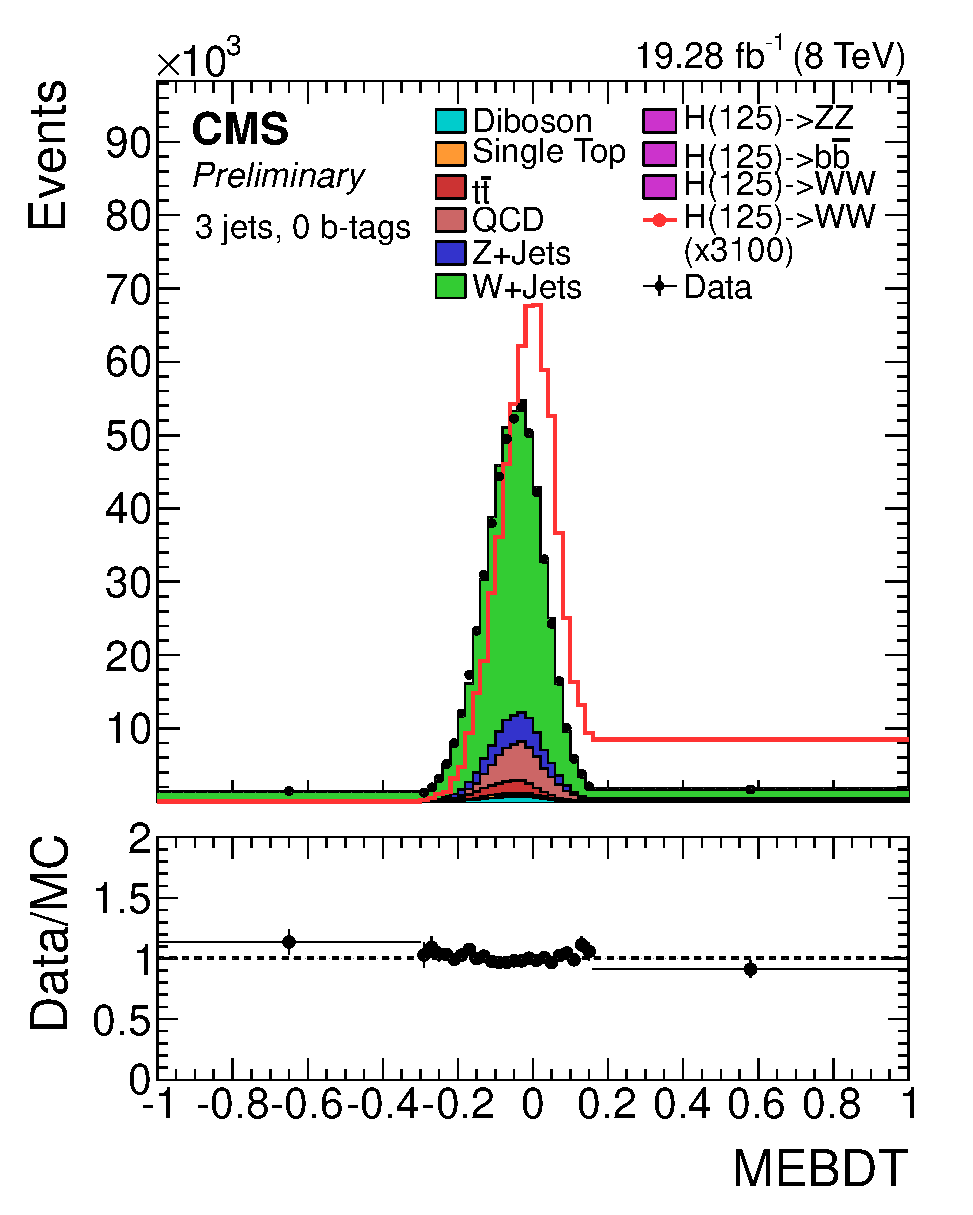
\includegraphics[width=\textwidth]{\figpath/Appendix5/jets2/muon/MEBDT_muon.eps}
        \caption{}
        \label{fig:MEBDT_jets2_muon_noSys}
    \end{subfigure}
    \caption{(a) The BDT response plot from TMVA for the training with only matrix element probabilities in the 2 jet bin for the combined lepton channel. Validation plot for the BDT in the 2 jet bin for the (b) electron and (c) muon channels. Only statistical uncertainties are shown in the validation plots.}
    \label{fig:MEBDT_Comparison_jets2}
\end{figure}

\begin{figure}[!hbt]
    \centering
    \begin{subfigure}[t]{0.317\textwidth}
        \includegraphics[width=\textwidth]{\figpath/Appendix5/jets3/2015_07_17_TMVA_output_jets3_eq0tag_both_HToWW_WJets_allEvtProbs_0KinVar/mva_BDT.pdf}
        \caption{}
        \label{fig:MEBDT_Response_3j0B_TMVA}
    \end{subfigure}
    \begin{subfigure}[t]{0.317\textwidth}
        \includegraphics[width=\textwidth]{\figpath/Appendix5/jets3/electron/MEBDT_electron.eps}
        \caption{}
        \label{fig:MEBDT_jets3_electron_noSys}
    \end{subfigure}
    \begin{subfigure}[t]{0.317\textwidth}
        \includegraphics[width=\textwidth]{\figpath/Appendix5/jets3/muon/MEBDT_muon.eps}
        \caption{}
        \label{fig:MEBDT_jets3_muon_noSys}
    \end{subfigure}
    \caption{(a) The BDT response plot from TMVA for the training with only matrix element probabilities in the 3 jet bin for the combined lepton channel. Validation plot for the BDT in the 3 jet bin for the (b) electron and (c) muon channels. Only statistical uncertainties are shown in the validation plots.}
    \label{fig:MEBDT_Comparison_jets3}
\end{figure}

\begin{figure}[!hbt]
    \centering
    \begin{subfigure}[t]{0.317\textwidth}
        \includegraphics[width=\textwidth]{\figpath/Appendix5/jets4/2015_07_17_TMVA_output_jets4_eq0tag_both_HToWW_WJets_allEvtProbs_0KinVar/mva_BDT.pdf}
        \caption{}
        \label{fig:MEBDT_Response_4j0B_TMVA}
    \end{subfigure}
    \begin{subfigure}[t]{0.317\textwidth}
        \includegraphics[width=\textwidth]{\figpath/Appendix5/jets4/electron/MEBDT_electron.eps}
        \caption{}
        \label{fig:MEBDT_jets4_electron_noSys}
    \end{subfigure}
    \begin{subfigure}[t]{0.317\textwidth}
        \includegraphics[width=\textwidth]{\figpath/Appendix5/jets4/muon/MEBDT_muon.eps}
        \caption{}
        \label{fig:MEBDT_jets4_muon_noSys}
    \end{subfigure}
    \caption{(a) The BDT response plot from TMVA for the training with only matrix element probabilities in the $\geqslant$4 jet bin for the combined lepton channel. Validation plot for the BDT in the $\geqslant$4 jet bin for the (b) electron and (c) muon channels. Only statistical uncertainties are shown in the validation plots.}
    \label{fig:MEBDT_Comparison_jets4}
\end{figure}

\begin{figure}[!hbt]
    \centering
    \begin{subfigure}[t]{0.317\textwidth}
        \includegraphics[width=\textwidth]{\figpath/Appendix5/jets2/2015_07_17_TMVA_output_jets2_eq0tag_both_HToWW_WJets_noEvtProbs_12KinVar/mva_BDT.pdf}
        \caption{}
        \label{fig:KinMEBDT_Response_2j0B_TMVA}
    \end{subfigure}
    \begin{subfigure}[t]{0.317\textwidth}
        \includegraphics[width=\textwidth]{\figpath/Appendix5/jets2/electron/KinMEBDT_electron.eps}
        \caption{}
        \label{fig:KinMEBDT_jets2_electron_noSys}
    \end{subfigure}
    \begin{subfigure}[t]{0.317\textwidth}
        \includegraphics[width=\textwidth]{\figpath/Appendix5/jets2/muon/KinMEBDT_muon.eps}
        \caption{}
        \label{fig:KinMEBDT_jets2_muon_noSys}
    \end{subfigure}
    \caption{(a) The BDT response plot from TMVA for the training with the kinematic variables and the ME BDT in the 2 jet bin for the combined lepton channel. Validation plot for the BDT in the 2 jet bin for the (b) electron and (c) muon channels. Only statistical uncertainties are shown in the validation plots.}
    \label{fig:KinMEBDT_Comparison_jets2}
\end{figure}

\begin{figure}[!hbt]
    \centering
    \begin{subfigure}[t]{0.317\textwidth}
        \includegraphics[width=\textwidth]{\figpath/Appendix5/jets3/2015_07_17_TMVA_output_jets3_eq0tag_both_HToWW_WJets_noEvtProbs_14KinVar/mva_BDT.pdf}
        \caption{}
        \label{fig:KinMEBDT_Response_3j0B_TMVA}
    \end{subfigure}
    \begin{subfigure}[t]{0.317\textwidth}
        \includegraphics[width=\textwidth]{\figpath/Appendix5/jets3/electron/KinMEBDT_electron.eps}
        \caption{}
        \label{fig:KinMEBDT_jets3_electron_noSys}
    \end{subfigure}
    \begin{subfigure}[t]{0.317\textwidth}
        \includegraphics[width=\textwidth]{\figpath/Appendix5/jets3/muon/KinMEBDT_muon.eps}
        \caption{}
        \label{fig:KinMEBDT_jets3_muon_noSys}
    \end{subfigure}
    \caption{(a) The BDT response plot from TMVA for the training with the kinematic variables and the ME BDT in the 3 jet bin for the combined lepton channel. Validation plot for the BDT in the 3 jet bin for the (b) electron and (c) muon channels. Only statistical uncertainties are shown in the validation plots.}
    \label{fig:KinMEBDT_Comparison_jets3}
\end{figure}

\begin{figure}[!hbt]
    \centering
    \begin{subfigure}[t]{0.317\textwidth}
        \includegraphics[width=\textwidth]{\figpath/Appendix5/jets4/2015_07_17_TMVA_output_jets4_eq0tag_both_HToWW_WJets_noEvtProbs_8KinVar/mva_BDT.pdf}
        \caption{}
        \label{fig:KinMEBDT_Response_4j0B_TMVA}
    \end{subfigure}
    \begin{subfigure}[t]{0.317\textwidth}
        \includegraphics[width=\textwidth]{\figpath/Appendix5/jets4/electron/KinMEBDT_electron.eps}
        \caption{}
        \label{fig:KinMEBDT_jets4_electron_noSys}
    \end{subfigure}
    \begin{subfigure}[t]{0.317\textwidth}
        \includegraphics[width=\textwidth]{\figpath/Appendix5/jets4/muon/KinMEBDT_muon.eps}
        \caption{}
        \label{fig:KinMEBDT_jets4_muon_noSys}
    \end{subfigure}
    \caption{(a) The BDT response plot from TMVA for the training with the kinematic variables and the ME BDT in the $\geqslant$4 jet bin for the combined lepton channel. Validation plot for the BDT in the $\geqslant$4 jet bin for the (b) electron and (c) muon channels. Only statistical uncertainties are shown in the validation plots.}
    \label{fig:KinMEBDT_Comparison_jets4}
\end{figure}
\clearpage







\section{Correlations}
\label{appendix:BDT_Correlations}

\begin{figure}[!hbt]
    \centering
    \begin{subfigure}[t]{0.48\textwidth}
        \includegraphics[width=\textwidth]{\figpath/Chapter5/BDT_Performance_Plots/CorrelationMatrixS_2j0B.png}
        \caption{}
        \label{fig:KinBDT_jets2_CorrelationS}
    \end{subfigure}
    \begin{subfigure}[t]{0.48\textwidth}
        \includegraphics[width=\textwidth]{\figpath/Chapter5/BDT_Performance_Plots/CorrelationMatrixB_2j0B.png}
        \caption{}
        \label{fig:KinBDT_jets2_CorrelationB}
    \end{subfigure}
    \caption{Correlation plots for (a) signal and (b) background for the BDT trained with only kinematic variables in the 2 jet bin.}
    \label{fig:KinBDT_jets2_Correlations}
\end{figure}

\begin{figure}[!hbt]
    \centering
    \begin{subfigure}[t]{0.48\textwidth}
        \includegraphics[width=\textwidth]{\figpath/Chapter5/BDT_Performance_Plots/CorrelationMatrixS_3j0B.png}
        \caption{}
        \label{fig:KinBDT_jets3_CorrelationS}
    \end{subfigure}
    \begin{subfigure}[t]{0.48\textwidth}
        \includegraphics[width=\textwidth]{\figpath/Chapter5/BDT_Performance_Plots/CorrelationMatrixB_3j0B.png}
        \caption{}
        \label{fig:KinBDT_jets3_CorrelationB}
    \end{subfigure}
    \caption{Correlation plots for (a) signal and (b) background for the BDT trained with only kinematic variables in the 3 jet bin.}
    \label{fig:KinBDT_jets3_Correlations}
\end{figure}

\begin{figure}[!hbt]
    \centering
    \begin{subfigure}[t]{0.48\textwidth}
        \includegraphics[width=\textwidth]{\figpath/Chapter5/BDT_Performance_Plots/CorrelationMatrixS_4j0B.png}
        \caption{}
        \label{fig:KinBDT_jets4_CorrelationS}
    \end{subfigure}
    \begin{subfigure}[t]{0.48\textwidth}
        \includegraphics[width=\textwidth]{\figpath/Chapter5/BDT_Performance_Plots/CorrelationMatrixB_4j0B.png}
        \caption{}
        \label{fig:KinBDT_jets4_CorrelationB}
    \end{subfigure}
    \caption{Correlation plots for (a) signal and (b) background for the BDT trained with only kinematic variables in the $\geqslant$4 jet bin.}
    \label{fig:KinBDT_jets4_Correlations}
\end{figure}

\begin{figure}[!hbt]
    \centering
    \begin{subfigure}[t]{0.48\textwidth}
        \includegraphics[width=\textwidth]{\figpath/Appendix5/jets2/2015_07_17_TMVA_output_jets2_eq0tag_both_HToWW_WJets_allEvtProbs_0KinVar/CorrelationMatrixS.pdf}
        \caption{}
        \label{fig:MEBDT_jets2_CorrelationS}
    \end{subfigure}
    \begin{subfigure}[t]{0.48\textwidth}
        \includegraphics[width=\textwidth]{\figpath/Appendix5/jets2/2015_07_17_TMVA_output_jets2_eq0tag_both_HToWW_WJets_allEvtProbs_0KinVar/CorrelationMatrixB.pdf}
        \caption{}
        \label{fig:MEBDT_jets2_CorrelationB}
    \end{subfigure}
    \caption{Correlation plots for (a) signal and (b) background for the BDT trained with only matrix elements variables in the 2 jet bin.}
    \label{fig:MEBDT_jets2_Correlations}
\end{figure}

\begin{figure}[!hbt]
    \centering
    \begin{subfigure}[t]{0.48\textwidth}
        \includegraphics[width=\textwidth]{\figpath/Appendix5/jets3/2015_07_17_TMVA_output_jets3_eq0tag_both_HToWW_WJets_allEvtProbs_0KinVar/CorrelationMatrixS.pdf}
        \caption{}
        \label{fig:MEBDT_jets3_CorrelationS}
    \end{subfigure}
    \begin{subfigure}[t]{0.48\textwidth}
        \includegraphics[width=\textwidth]{\figpath/Appendix5/jets3/2015_07_17_TMVA_output_jets3_eq0tag_both_HToWW_WJets_allEvtProbs_0KinVar/CorrelationMatrixB.pdf}
        \caption{}
        \label{fig:MEBDT_jets3_CorrelationB}
    \end{subfigure}
    \caption{Correlation plots for (a) signal and (b) background for the BDT trained with only matrix elements variables in the 3 jet bin.}
    \label{fig:MEBDT_jets3_Correlations}
\end{figure}

\begin{figure}[!hbt]
    \centering
    \begin{subfigure}[t]{0.48\textwidth}
        \includegraphics[width=\textwidth]{\figpath/Appendix5/jets4/2015_07_17_TMVA_output_jets4_eq0tag_both_HToWW_WJets_allEvtProbs_0KinVar/CorrelationMatrixS.pdf}
        \caption{}
        \label{fig:MEBDT_jets4_CorrelationS}
    \end{subfigure}
    \begin{subfigure}[t]{0.48\textwidth}
        \includegraphics[width=\textwidth]{\figpath/Appendix5/jets4/2015_07_17_TMVA_output_jets4_eq0tag_both_HToWW_WJets_allEvtProbs_0KinVar/CorrelationMatrixB.pdf}
        \caption{}
        \label{fig:MEBDT_jets4_CorrelationB}
    \end{subfigure}
    \caption{Correlation plots for (a) signal and (b) background for the BDT trained with only matrix elements variables in the $\geqslant$4 jet bin.}
    \label{fig:MEBDT_jets4_Correlations}
\end{figure}

\begin{figure}[!hbt]
    \centering
    \begin{subfigure}[t]{0.48\textwidth}
        \includegraphics[width=\textwidth]{\figpath/Appendix5/jets2/2015_07_17_TMVA_output_jets2_eq0tag_both_HToWW_WJets_noEvtProbs_12KinVar/CorrelationMatrixS.pdf}
        \caption{}
        \label{fig:KinMEBDT_jets2_CorrelationS}
    \end{subfigure}
    \begin{subfigure}[t]{0.48\textwidth}
        \includegraphics[width=\textwidth]{\figpath/Appendix5/jets2/2015_07_17_TMVA_output_jets2_eq0tag_both_HToWW_WJets_noEvtProbs_12KinVar/CorrelationMatrixB.pdf}
        \caption{}
        \label{fig:KinMEBDT_jets2_CorrelationB}
    \end{subfigure}
    \caption{Correlation plots for (a) signal and (b) background for the BDT trained with both the kinematic variables and the ME BDT in the 2 jet bin.}
    \label{fig:KinMEBDT_jets2_Correlations}
\end{figure}

\begin{figure}[!hbt]
    \centering
    \begin{subfigure}[t]{0.48\textwidth}
        \includegraphics[width=\textwidth]{\figpath/Appendix5/jets3/2015_07_17_TMVA_output_jets3_eq0tag_both_HToWW_WJets_noEvtProbs_14KinVar/CorrelationMatrixS.pdf}
        \caption{}
        \label{fig:KinMEBDT_jets3_CorrelationS}
    \end{subfigure}
    \begin{subfigure}[t]{0.48\textwidth}
        \includegraphics[width=\textwidth]{\figpath/Appendix5/jets3/2015_07_17_TMVA_output_jets3_eq0tag_both_HToWW_WJets_noEvtProbs_14KinVar/CorrelationMatrixB.pdf}
        \caption{}
        \label{fig:KinMEBDT_jets3_CorrelationB}
    \end{subfigure}
    \caption{Correlation plots for (a) signal and (b) background for the BDT trained with both the kinematic variables and the ME BDT in the 3 jet bin.}
    \label{fig:KinMEBDT_jets3_Correlations}
\end{figure}

\begin{figure}[!hbt]
    \centering
    \begin{subfigure}[t]{0.48\textwidth}
        \includegraphics[width=\textwidth]{\figpath/Appendix5/jets4/2015_07_17_TMVA_output_jets4_eq0tag_both_HToWW_WJets_noEvtProbs_8KinVar/CorrelationMatrixS.pdf}
        \caption{}
        \label{fig:KinMEBDT_jets4_CorrelationS}
    \end{subfigure}
    \begin{subfigure}[t]{0.48\textwidth}
        \includegraphics[width=\textwidth]{\figpath/Appendix5/jets4/2015_07_17_TMVA_output_jets4_eq0tag_both_HToWW_WJets_noEvtProbs_8KinVar/CorrelationMatrixB.pdf}
        \caption{}
        \label{fig:KinMEBDT_jets4_CorrelationB}
    \end{subfigure}
    \caption{Correlation plots for (a) signal and (b) background for the BDT trained with both the kinematic variables and the ME BDT in the $\geqslant$4 jet bin.}
    \label{fig:KinMEBDT_jets4_Correlations}
\end{figure}
\clearpage







\section{ROC Curves}
\label{appendix:BDT_ROC_curves}
\begin{figure}[!hbt]
    \centering
    \begin{subfigure}[t]{0.316\textwidth}
        \includegraphics[width=\textwidth]{\figpath/Appendix5/jets2/2015_07_17_TMVA_output_jets2_eq0tag_both_HToWW_WJets_noEvtProbs_11KinVar/rejBvsS_BDT_simple.pdf}
        \caption{}
        \label{fig:KinBDT_ROC_jets2}
    \end{subfigure}
    \begin{subfigure}[t]{0.316\textwidth}
        \includegraphics[width=\textwidth]{\figpath/Appendix5/jets3/2015_07_17_TMVA_output_jets3_eq0tag_both_HToWW_WJets_noEvtProbs_13KinVar/rejBvsS_BDT_simple.pdf}
        \caption{}
        \label{fig:KinBDT_ROC_jets3}
    \end{subfigure}
    \begin{subfigure}[t]{0.316\textwidth}
        \includegraphics[width=\textwidth]{\figpath/Appendix5/jets4/2015_07_17_TMVA_output_jets4_eq0tag_both_HToWW_WJets_noEvtProbs_7KinVar/rejBvsS_BDT_simple.pdf}
        \caption{}
        \label{fig:KinBDT_ROC_jets4}
    \end{subfigure}

    \begin{subfigure}[t]{0.316\textwidth}
        \includegraphics[width=\textwidth]{\figpath/Appendix5/jets2/2015_07_17_TMVA_output_jets2_eq0tag_both_HToWW_WJets_allEvtProbs_0KinVar/rejBvsS_BDT_simple.pdf}
        \caption{}
        \label{fig:MEBDT_ROC_jets2}
    \end{subfigure}
    \begin{subfigure}[t]{0.316\textwidth}
        \includegraphics[width=\textwidth]{\figpath/Appendix5/jets3/2015_07_17_TMVA_output_jets3_eq0tag_both_HToWW_WJets_allEvtProbs_0KinVar/rejBvsS_BDT_simple.pdf}
        \caption{}
        \label{fig:MEBDT_ROC_jets3}
    \end{subfigure}
    \begin{subfigure}[t]{0.316\textwidth}
        \includegraphics[width=\textwidth]{\figpath/Appendix5/jets4/2015_07_17_TMVA_output_jets4_eq0tag_both_HToWW_WJets_allEvtProbs_0KinVar/rejBvsS_BDT_simple.pdf}
        \caption{}
        \label{fig:MEBDT_ROC_jets4}
    \end{subfigure}

    \begin{subfigure}[t]{0.316\textwidth}
        \includegraphics[width=\textwidth]{\figpath/Appendix5/jets2/2015_07_17_TMVA_output_jets2_eq0tag_both_HToWW_WJets_noEvtProbs_12KinVar/rejBvsS_BDT_simple.pdf}
        \caption{}
        \label{fig:KinMEBDT_ROC_jets2}
    \end{subfigure}
    \begin{subfigure}[t]{0.316\textwidth}
        \includegraphics[width=\textwidth]{\figpath/Appendix5/jets3/2015_07_17_TMVA_output_jets3_eq0tag_both_HToWW_WJets_noEvtProbs_14KinVar/rejBvsS_BDT_simple.pdf}
        \caption{}
        \label{fig:KinMEBDT_ROC_jets3}
    \end{subfigure}
    \begin{subfigure}[t]{0.316\textwidth}
        \includegraphics[width=\textwidth]{\figpath/Appendix5/jets4/2015_07_17_TMVA_output_jets4_eq0tag_both_HToWW_WJets_noEvtProbs_8KinVar/rejBvsS_BDT_simple.pdf}
        \caption{}
        \label{fig:KinMEBDT_ROC_jets4}
    \end{subfigure}
    \caption{The receiver operating characteristic (ROC) curves for the various BDT trainings. The plots are ordered by jet bin from left to right, with the leftmost plot being the two-jet bin and the rightmost plot being the greater than or equal to four-jet bin. The top row contains the KinBDT plots while the middle and bottom rows contain the MEBDT and KinMEBDT plots, respectively.}
    \label{fig:BDT_ROC_all}
\end{figure}




\clearpage

%!TEX root = ../TAMUTemplate.tex
%%%%%%%%%%%%%%%%%%%%%%%%%%%%%%%%%%%%%%%%%%%%%%%%%%%
%
%  New template code for TAMU Theses and Dissertations starting Fall 2016.
%
%
%  Author: Sean Zachary Roberson 
%	 Version 3.16.09
%  Last updated 9/12/2016
%
%%%%%%%%%%%%%%%%%%%%%%%%%%%%%%%%%%%%%%%%%%%%%%%%%%%

%%%%%%%%%%%%%%%%%%%%%%%%%%%%%%%%%%%%%%%%%%%%%%%%%%%%%%%%%%%%%%%%%%%%%%
%%                           APPENDIX E 
%%%%%%%%%%%%%%%%%%%%%%%%%%%%%%%%%%%%%%%%%%%%%%%%%%%%%%%%%%%%%%%%%%%%%

\chapter{\texorpdfstring{\uppercase{Boosted Decision Trees}}{Boosted Decision Trees}}

\section{Inputs}
\label{appendix:BDT_Inputs}
\section{Outputs}
\label{appendix:BDT_Outputs}
\section{Correlations}
\label{appendix:BDT_Correlations}


%!TEX root = ../TAMUTemplate.tex
%%%%%%%%%%%%%%%%%%%%%%%%%%%%%%%%%%%%%%%%%%%%%%%%%%%
%
%  New template code for TAMU Theses and Dissertations starting Fall 2016.
%
%
%  Author: Sean Zachary Roberson 
%	 Version 3.16.09 
%  Last updated 9/12/2016
%
%%%%%%%%%%%%%%%%%%%%%%%%%%%%%%%%%%%%%%%%%%%%%%%%%%%

%%%%%%%%%%%%%%%%%%%%%%%%%%%%%%%%%%%%%%%%%%%%%%%%%%%%%%%%%%%%%%%%%%%%%%
%%                           APPENDIX F
%%%%%%%%%%%%%%%%%%%%%%%%%%%%%%%%%%%%%%%%%%%%%%%%%%%%%%%%%%%%%%%%%%%%%

\chapter{\texorpdfstring{\uppercase {Comparison Plots}}{Comparison Plots}}
\label{appendix:comparison_plots}

\begin{figure}[!hbtp]
    \centering
    \begin{subfigure}[t]{0.317\textwidth}
        \includegraphics[width=\textwidth]{\figpath/Appendix6/jets2/electron/CosTheta_WH_electron.eps}
    \end{subfigure}
    \begin{subfigure}[t]{0.317\textwidth}
        \includegraphics[width=\textwidth]{\figpath/Appendix6/jets2/electron/CosTheta_j_electron.eps}
    \end{subfigure}
    \begin{subfigure}[t]{0.317\textwidth}
        \includegraphics[width=\textwidth]{\figpath/Appendix6/jets2/electron/CosTheta_l_electron.eps}
    \end{subfigure}

    \begin{subfigure}[t]{0.317\textwidth}
        \includegraphics[width=\textwidth]{\figpath/Appendix6/jets2/electron/DeltaEtaJ1J2_electron.eps}
    \end{subfigure}
    \begin{subfigure}[t]{0.317\textwidth}
        \includegraphics[width=\textwidth]{\figpath/Appendix6/jets2/electron/DeltaPhi_J1J2_electron.eps}
    \end{subfigure}
    \begin{subfigure}[t]{0.317\textwidth}
        \includegraphics[width=\textwidth]{\figpath/Appendix6/jets2/electron/minDPhiLepJet_electron.eps}
    \end{subfigure}

    \begin{subfigure}[t]{0.317\textwidth}
        \includegraphics[width=\textwidth]{\figpath/Appendix6/jets2/electron/dPhiMETJet_electron.eps}
    \end{subfigure}
    \begin{subfigure}[t]{0.317\textwidth}
        \includegraphics[width=\textwidth]{\figpath/Appendix6/jets2/electron/dPhiMETLep_electron.eps}
    \end{subfigure}
    \begin{subfigure}[t]{0.317\textwidth}
        \includegraphics[width=\textwidth]{\figpath/Appendix6/jets2/electron/dRlepjj_electron.eps}
    \end{subfigure}
    \caption{Data-to-MC comparison plots for the 2-jet electron channel.}
    \label{fig:comparison_plots_jets2_electron_1}
\end{figure}

\begin{figure}[!hbtp]
    \centering
    \begin{subfigure}[t]{0.317\textwidth}
        \includegraphics[width=\textwidth]{\figpath/Appendix6/jets2/electron/LeptPt_electron.eps}
    \end{subfigure}
    \begin{subfigure}[t]{0.317\textwidth}
        \includegraphics[width=\textwidth]{\figpath/Appendix6/jets2/electron/ht_electron.eps}
    \end{subfigure}
    \begin{subfigure}[t]{0.317\textwidth}
        \includegraphics[width=\textwidth]{\figpath/Appendix6/jets2/electron/leptonEtaCharge_electron.eps}
    \end{subfigure}

    \begin{subfigure}[t]{0.317\textwidth}
        \includegraphics[width=\textwidth]{\figpath/Appendix6/jets2/electron/jet1dRLep_electron.eps}
    \end{subfigure}
    \begin{subfigure}[t]{0.317\textwidth}
        \includegraphics[width=\textwidth]{\figpath/Appendix6/jets2/electron/jet2dRLep_electron.eps}
    \end{subfigure}
    \begin{subfigure}[t]{0.317\textwidth}
        \includegraphics[width=\textwidth]{\figpath/Appendix6/jets2/electron/jet3dRLep_electron.eps}
    \end{subfigure}

    \begin{subfigure}[t]{0.317\textwidth}
        \includegraphics[width=\textwidth]{\figpath/Appendix6/jets2/electron/WmT_electron.eps}
    \end{subfigure}
    \begin{subfigure}[t]{0.317\textwidth}
        \includegraphics[width=\textwidth]{\figpath/Appendix6/jets2/electron/Ptlnujj_electron.eps}
    \end{subfigure}
    \begin{subfigure}[t]{0.317\textwidth}
        \includegraphics[width=\textwidth]{\figpath/Appendix6/jets2/electron/Mlvjj_electron.eps}
    \end{subfigure}
    \caption{Data-to-MC comparison plots for the 2-jet electron channel.}
    \label{fig:comparison_plots_jets2_electron_2}
\end{figure}
















\begin{figure}[!hbtp]
    \centering
    \begin{subfigure}[t]{0.317\textwidth}
        \includegraphics[width=\textwidth]{\figpath/Appendix6/jets3/electron/CosTheta_WH_electron.eps}
    \end{subfigure}
    \begin{subfigure}[t]{0.317\textwidth}
        \includegraphics[width=\textwidth]{\figpath/Appendix6/jets3/electron/CosTheta_j_electron.eps}
    \end{subfigure}
    \begin{subfigure}[t]{0.317\textwidth}
        \includegraphics[width=\textwidth]{\figpath/Appendix6/jets3/electron/CosTheta_l_electron.eps}
    \end{subfigure}

    \begin{subfigure}[t]{0.317\textwidth}
        \includegraphics[width=\textwidth]{\figpath/Appendix6/jets3/electron/DeltaEtaJ1J2_electron.eps}
    \end{subfigure}
    \begin{subfigure}[t]{0.317\textwidth}
        \includegraphics[width=\textwidth]{\figpath/Appendix6/jets3/electron/DeltaPhi_J1J2_electron.eps}
    \end{subfigure}
    \begin{subfigure}[t]{0.317\textwidth}
        \includegraphics[width=\textwidth]{\figpath/Appendix6/jets3/electron/minDPhiLepJet_electron.eps}
    \end{subfigure}

    \begin{subfigure}[t]{0.317\textwidth}
        \includegraphics[width=\textwidth]{\figpath/Appendix6/jets3/electron/dPhiMETJet_electron.eps}
    \end{subfigure}
    \begin{subfigure}[t]{0.317\textwidth}
        \includegraphics[width=\textwidth]{\figpath/Appendix6/jets3/electron/dPhiMETLep_electron.eps}
    \end{subfigure}
    \begin{subfigure}[t]{0.317\textwidth}
        \includegraphics[width=\textwidth]{\figpath/Appendix6/jets3/electron/dRlepjj_electron.eps}
    \end{subfigure}
    \caption{Data-to-MC comparison plots for the 3-jet electron channel.}
    \label{fig:comparison_plots_jets3_electron_1}
\end{figure}

\begin{figure}[!hbtp]
    \centering
    \begin{subfigure}[t]{0.317\textwidth}
        \includegraphics[width=\textwidth]{\figpath/Appendix6/jets3/electron/LeptPt_electron.eps}
    \end{subfigure}
    \begin{subfigure}[t]{0.317\textwidth}
        \includegraphics[width=\textwidth]{\figpath/Appendix6/jets3/electron/ht_electron.eps}
    \end{subfigure}
    \begin{subfigure}[t]{0.317\textwidth}
        \includegraphics[width=\textwidth]{\figpath/Appendix6/jets3/electron/leptonEtaCharge_electron.eps}
    \end{subfigure}

    \begin{subfigure}[t]{0.317\textwidth}
        \includegraphics[width=\textwidth]{\figpath/Appendix6/jets3/electron/jet1dRLep_electron.eps}
    \end{subfigure}
    \begin{subfigure}[t]{0.317\textwidth}
        \includegraphics[width=\textwidth]{\figpath/Appendix6/jets3/electron/jet2dRLep_electron.eps}
    \end{subfigure}
    \begin{subfigure}[t]{0.317\textwidth}
        \includegraphics[width=\textwidth]{\figpath/Appendix6/jets3/electron/jet3dRLep_electron.eps}
    \end{subfigure}

    \begin{subfigure}[t]{0.317\textwidth}
        \includegraphics[width=\textwidth]{\figpath/Appendix6/jets3/electron/WmT_electron.eps}
    \end{subfigure}
    \begin{subfigure}[t]{0.317\textwidth}
        \includegraphics[width=\textwidth]{\figpath/Appendix6/jets3/electron/Ptlnujj_electron.eps}
    \end{subfigure}
    \begin{subfigure}[t]{0.317\textwidth}
        \includegraphics[width=\textwidth]{\figpath/Appendix6/jets3/electron/Mlvjj_electron.eps}
    \end{subfigure}
    \caption{Data-to-MC comparison plots for the 3-jet electron channel.}
    \label{fig:comparison_plots_jets3_electron_2}
\end{figure}















\begin{figure}[!hbtp]
    \centering
    \begin{subfigure}[t]{0.317\textwidth}
        \includegraphics[width=\textwidth]{\figpath/Appendix6/jets4/electron/CosTheta_WH_electron.eps}
    \end{subfigure}
    \begin{subfigure}[t]{0.317\textwidth}
        \includegraphics[width=\textwidth]{\figpath/Appendix6/jets4/electron/CosTheta_j_electron.eps}
    \end{subfigure}
    \begin{subfigure}[t]{0.317\textwidth}
        \includegraphics[width=\textwidth]{\figpath/Appendix6/jets4/electron/CosTheta_l_electron.eps}
    \end{subfigure}

    \begin{subfigure}[t]{0.317\textwidth}
        \includegraphics[width=\textwidth]{\figpath/Appendix6/jets4/electron/DeltaEtaJ1J2_electron.eps}
    \end{subfigure}
    \begin{subfigure}[t]{0.317\textwidth}
        \includegraphics[width=\textwidth]{\figpath/Appendix6/jets4/electron/DeltaPhi_J1J2_electron.eps}
    \end{subfigure}
    \begin{subfigure}[t]{0.317\textwidth}
        \includegraphics[width=\textwidth]{\figpath/Appendix6/jets4/electron/minDPhiLepJet_electron.eps}
    \end{subfigure}

    \begin{subfigure}[t]{0.317\textwidth}
        \includegraphics[width=\textwidth]{\figpath/Appendix6/jets4/electron/dPhiMETJet_electron.eps}
    \end{subfigure}
    \begin{subfigure}[t]{0.317\textwidth}
        \includegraphics[width=\textwidth]{\figpath/Appendix6/jets4/electron/dPhiMETLep_electron.eps}
    \end{subfigure}
    \begin{subfigure}[t]{0.317\textwidth}
        \includegraphics[width=\textwidth]{\figpath/Appendix6/jets4/electron/dRlepjj_electron.eps}
    \end{subfigure}
    \caption{Data-to-MC comparison plots for the $\geqslant$4-jet electron channel.}
    \label{fig:comparison_plots_jets4_electron_1}
\end{figure}

\begin{figure}[!hbtp]
    \centering
    \begin{subfigure}[t]{0.317\textwidth}
        \includegraphics[width=\textwidth]{\figpath/Appendix6/jets4/electron/LeptPt_electron.eps}
    \end{subfigure}
    \begin{subfigure}[t]{0.317\textwidth}
        \includegraphics[width=\textwidth]{\figpath/Appendix6/jets4/electron/ht_electron.eps}
    \end{subfigure}
    \begin{subfigure}[t]{0.317\textwidth}
        \includegraphics[width=\textwidth]{\figpath/Appendix6/jets4/electron/leptonEtaCharge_electron.eps}
    \end{subfigure}

    \begin{subfigure}[t]{0.317\textwidth}
        \includegraphics[width=\textwidth]{\figpath/Appendix6/jets4/electron/jet1dRLep_electron.eps}
    \end{subfigure}
    \begin{subfigure}[t]{0.317\textwidth}
        \includegraphics[width=\textwidth]{\figpath/Appendix6/jets4/electron/jet2dRLep_electron.eps}
    \end{subfigure}
    \begin{subfigure}[t]{0.317\textwidth}
        \includegraphics[width=\textwidth]{\figpath/Appendix6/jets4/electron/jet3dRLep_electron.eps}
    \end{subfigure}

    \begin{subfigure}[t]{0.317\textwidth}
        \includegraphics[width=\textwidth]{\figpath/Appendix6/jets4/electron/WmT_electron.eps}
    \end{subfigure}
    \begin{subfigure}[t]{0.317\textwidth}
        \includegraphics[width=\textwidth]{\figpath/Appendix6/jets4/electron/Ptlnujj_electron.eps}
    \end{subfigure}
    \begin{subfigure}[t]{0.317\textwidth}
        \includegraphics[width=\textwidth]{\figpath/Appendix6/jets4/electron/Mlvjj_electron.eps}
    \end{subfigure}
    \caption{Data-to-MC comparison plots for the $\geqslant$4-jet electron channel.}
    \label{fig:comparison_plots_jets4_electron_2}
\end{figure}
























\begin{figure}[!hbtp]
    \centering
    \begin{subfigure}[t]{0.317\textwidth}
        \includegraphics[width=\textwidth]{\figpath/Appendix6/jets2/muon/CosTheta_WH_muon.eps}
    \end{subfigure}
    \begin{subfigure}[t]{0.317\textwidth}
        \includegraphics[width=\textwidth]{\figpath/Appendix6/jets2/muon/CosTheta_j_muon.eps}
    \end{subfigure}
    \begin{subfigure}[t]{0.317\textwidth}
        \includegraphics[width=\textwidth]{\figpath/Appendix6/jets2/muon/CosTheta_l_muon.eps}
    \end{subfigure}

    \begin{subfigure}[t]{0.317\textwidth}
        \includegraphics[width=\textwidth]{\figpath/Appendix6/jets2/muon/DeltaEtaJ1J2_muon.eps}
    \end{subfigure}
    \begin{subfigure}[t]{0.317\textwidth}
        \includegraphics[width=\textwidth]{\figpath/Appendix6/jets2/muon/DeltaPhi_J1J2_muon.eps}
    \end{subfigure}
    \begin{subfigure}[t]{0.317\textwidth}
        \includegraphics[width=\textwidth]{\figpath/Appendix6/jets2/muon/minDPhiLepJet_muon.eps}
    \end{subfigure}

    \begin{subfigure}[t]{0.317\textwidth}
        \includegraphics[width=\textwidth]{\figpath/Appendix6/jets2/muon/dPhiMETJet_muon.eps}
    \end{subfigure}
    \begin{subfigure}[t]{0.317\textwidth}
        \includegraphics[width=\textwidth]{\figpath/Appendix6/jets2/muon/dPhiMETLep_muon.eps}
    \end{subfigure}
    \begin{subfigure}[t]{0.317\textwidth}
        \includegraphics[width=\textwidth]{\figpath/Appendix6/jets2/muon/dRlepjj_muon.eps}
    \end{subfigure}
    \caption{Data-to-MC comparison plots for the 2-jet muon channel.}
    \label{fig:comparison_plots_jets2_muon_1}
\end{figure}

\begin{figure}[!hbtp]
    \centering
    \begin{subfigure}[t]{0.317\textwidth}
        \includegraphics[width=\textwidth]{\figpath/Appendix6/jets2/muon/LeptPt_muon.eps}
    \end{subfigure}
    \begin{subfigure}[t]{0.317\textwidth}
        \includegraphics[width=\textwidth]{\figpath/Appendix6/jets2/muon/ht_muon.eps}
    \end{subfigure}
    \begin{subfigure}[t]{0.317\textwidth}
        \includegraphics[width=\textwidth]{\figpath/Appendix6/jets2/muon/leptonEtaCharge_muon.eps}
    \end{subfigure}

    \begin{subfigure}[t]{0.317\textwidth}
        \includegraphics[width=\textwidth]{\figpath/Appendix6/jets2/muon/jet1dRLep_muon.eps}
    \end{subfigure}
    \begin{subfigure}[t]{0.317\textwidth}
        \includegraphics[width=\textwidth]{\figpath/Appendix6/jets2/muon/jet2dRLep_muon.eps}
    \end{subfigure}
    \begin{subfigure}[t]{0.317\textwidth}
        \includegraphics[width=\textwidth]{\figpath/Appendix6/jets2/muon/jet3dRLep_muon.eps}
    \end{subfigure}

    \begin{subfigure}[t]{0.317\textwidth}
        \includegraphics[width=\textwidth]{\figpath/Appendix6/jets2/muon/WmT_muon.eps}
    \end{subfigure}
    \begin{subfigure}[t]{0.317\textwidth}
        \includegraphics[width=\textwidth]{\figpath/Appendix6/jets2/muon/Ptlnujj_muon.eps}
    \end{subfigure}
    \begin{subfigure}[t]{0.317\textwidth}
        \includegraphics[width=\textwidth]{\figpath/Appendix6/jets2/muon/Mlvjj_muon.eps}
    \end{subfigure}
    \caption{Data-to-MC comparison plots for the 2-jet muon channel.}
    \label{fig:comparison_plots_jets2_muon_2}
\end{figure}
















\begin{figure}[!hbtp]
    \centering
    \begin{subfigure}[t]{0.317\textwidth}
        \includegraphics[width=\textwidth]{\figpath/Appendix6/jets3/muon/CosTheta_WH_muon.eps}
    \end{subfigure}
    \begin{subfigure}[t]{0.317\textwidth}
        \includegraphics[width=\textwidth]{\figpath/Appendix6/jets3/muon/CosTheta_j_muon.eps}
    \end{subfigure}
    \begin{subfigure}[t]{0.317\textwidth}
        \includegraphics[width=\textwidth]{\figpath/Appendix6/jets3/muon/CosTheta_l_muon.eps}
    \end{subfigure}

    \begin{subfigure}[t]{0.317\textwidth}
        \includegraphics[width=\textwidth]{\figpath/Appendix6/jets3/muon/DeltaEtaJ1J2_muon.eps}
    \end{subfigure}
    \begin{subfigure}[t]{0.317\textwidth}
        \includegraphics[width=\textwidth]{\figpath/Appendix6/jets3/muon/DeltaPhi_J1J2_muon.eps}
    \end{subfigure}
    \begin{subfigure}[t]{0.317\textwidth}
        \includegraphics[width=\textwidth]{\figpath/Appendix6/jets3/muon/minDPhiLepJet_muon.eps}
    \end{subfigure}

    \begin{subfigure}[t]{0.317\textwidth}
        \includegraphics[width=\textwidth]{\figpath/Appendix6/jets3/muon/dPhiMETJet_muon.eps}
    \end{subfigure}
    \begin{subfigure}[t]{0.317\textwidth}
        \includegraphics[width=\textwidth]{\figpath/Appendix6/jets3/muon/dPhiMETLep_muon.eps}
    \end{subfigure}
    \begin{subfigure}[t]{0.317\textwidth}
        \includegraphics[width=\textwidth]{\figpath/Appendix6/jets3/muon/dRlepjj_muon.eps}
    \end{subfigure}
    \caption{Data-to-MC comparison plots for the 3-jet muon channel.}
    \label{fig:comparison_plots_jets3_muon_1}
\end{figure}

\begin{figure}[!hbtp]
    \centering
    \begin{subfigure}[t]{0.317\textwidth}
        \includegraphics[width=\textwidth]{\figpath/Appendix6/jets3/muon/LeptPt_muon.eps}
    \end{subfigure}
    \begin{subfigure}[t]{0.317\textwidth}
        \includegraphics[width=\textwidth]{\figpath/Appendix6/jets3/muon/ht_muon.eps}
    \end{subfigure}
    \begin{subfigure}[t]{0.317\textwidth}
        \includegraphics[width=\textwidth]{\figpath/Appendix6/jets3/muon/leptonEtaCharge_muon.eps}
    \end{subfigure}

    \begin{subfigure}[t]{0.317\textwidth}
        \includegraphics[width=\textwidth]{\figpath/Appendix6/jets3/muon/jet1dRLep_muon.eps}
    \end{subfigure}
    \begin{subfigure}[t]{0.317\textwidth}
        \includegraphics[width=\textwidth]{\figpath/Appendix6/jets3/muon/jet2dRLep_muon.eps}
    \end{subfigure}
    \begin{subfigure}[t]{0.317\textwidth}
        \includegraphics[width=\textwidth]{\figpath/Appendix6/jets3/muon/jet3dRLep_muon.eps}
    \end{subfigure}

    \begin{subfigure}[t]{0.317\textwidth}
        \includegraphics[width=\textwidth]{\figpath/Appendix6/jets3/muon/WmT_muon.eps}
    \end{subfigure}
    \begin{subfigure}[t]{0.317\textwidth}
        \includegraphics[width=\textwidth]{\figpath/Appendix6/jets3/muon/Ptlnujj_muon.eps}
    \end{subfigure}
    \begin{subfigure}[t]{0.317\textwidth}
        \includegraphics[width=\textwidth]{\figpath/Appendix6/jets3/muon/Mlvjj_muon.eps}
    \end{subfigure}
    \caption{Data-to-MC comparison plots for the 3-jet muon channel.}
    \label{fig:comparison_plots_jets3_muon_2}
\end{figure}















\begin{figure}[!hbtp]
    \centering
    \begin{subfigure}[t]{0.317\textwidth}
        \includegraphics[width=\textwidth]{\figpath/Appendix6/jets4/muon/CosTheta_WH_muon.eps}
    \end{subfigure}
    \begin{subfigure}[t]{0.317\textwidth}
        \includegraphics[width=\textwidth]{\figpath/Appendix6/jets4/muon/CosTheta_j_muon.eps}
    \end{subfigure}
    \begin{subfigure}[t]{0.317\textwidth}
        \includegraphics[width=\textwidth]{\figpath/Appendix6/jets4/muon/CosTheta_l_muon.eps}
    \end{subfigure}

    \begin{subfigure}[t]{0.317\textwidth}
        \includegraphics[width=\textwidth]{\figpath/Appendix6/jets4/muon/DeltaEtaJ1J2_muon.eps}
    \end{subfigure}
    \begin{subfigure}[t]{0.317\textwidth}
        \includegraphics[width=\textwidth]{\figpath/Appendix6/jets4/muon/DeltaPhi_J1J2_muon.eps}
    \end{subfigure}
    \begin{subfigure}[t]{0.317\textwidth}
        \includegraphics[width=\textwidth]{\figpath/Appendix6/jets4/muon/minDPhiLepJet_muon.eps}
    \end{subfigure}

    \begin{subfigure}[t]{0.317\textwidth}
        \includegraphics[width=\textwidth]{\figpath/Appendix6/jets4/muon/dPhiMETJet_muon.eps}
    \end{subfigure}
    \begin{subfigure}[t]{0.317\textwidth}
        \includegraphics[width=\textwidth]{\figpath/Appendix6/jets4/muon/dPhiMETLep_muon.eps}
    \end{subfigure}
    \begin{subfigure}[t]{0.317\textwidth}
        \includegraphics[width=\textwidth]{\figpath/Appendix6/jets4/muon/dRlepjj_muon.eps}
    \end{subfigure}
    \caption{Data-to-MC comparison plots for the $\geqslant$4-jet muon channel.}
    \label{fig:comparison_plots_jets4_muon_1}
\end{figure}

\begin{figure}[!hbtp]
    \centering
    \begin{subfigure}[t]{0.317\textwidth}
        \includegraphics[width=\textwidth]{\figpath/Appendix6/jets4/muon/LeptPt_muon.eps}
    \end{subfigure}
    \begin{subfigure}[t]{0.317\textwidth}
        \includegraphics[width=\textwidth]{\figpath/Appendix6/jets4/muon/ht_muon.eps}
    \end{subfigure}
    \begin{subfigure}[t]{0.317\textwidth}
        \includegraphics[width=\textwidth]{\figpath/Appendix6/jets4/muon/leptonEtaCharge_muon.eps}
    \end{subfigure}

    \begin{subfigure}[t]{0.317\textwidth}
        \includegraphics[width=\textwidth]{\figpath/Appendix6/jets4/muon/jet1dRLep_muon.eps}
    \end{subfigure}
    \begin{subfigure}[t]{0.317\textwidth}
        \includegraphics[width=\textwidth]{\figpath/Appendix6/jets4/muon/jet2dRLep_muon.eps}
    \end{subfigure}
    \begin{subfigure}[t]{0.317\textwidth}
        \includegraphics[width=\textwidth]{\figpath/Appendix6/jets4/muon/jet3dRLep_muon.eps}
    \end{subfigure}

    \begin{subfigure}[t]{0.317\textwidth}
        \includegraphics[width=\textwidth]{\figpath/Appendix6/jets4/muon/WmT_muon.eps}
    \end{subfigure}
    \begin{subfigure}[t]{0.317\textwidth}
        \includegraphics[width=\textwidth]{\figpath/Appendix6/jets4/muon/Ptlnujj_muon.eps}
    \end{subfigure}
    \begin{subfigure}[t]{0.317\textwidth}
        \includegraphics[width=\textwidth]{\figpath/Appendix6/jets4/muon/Mlvjj_muon.eps}
    \end{subfigure}
    \caption{Data-to-MC comparison plots for the $\geqslant$4-jet muon channel.}
    \label{fig:comparison_plots_jets4_muon_2}
\end{figure}





\pagebreak{}
\input{data/appendix7}

\end{appendices}


\end{document}
